% Revised Title and Main Document Structure
% Publication-ready with clearer terminology

\documentclass[11pt]{article}
% Shared preamble for the TSFM-PHM manuscript.
\usepackage[a4paper,margin=1in]{geometry}
\usepackage[T1]{fontenc}
\usepackage{lmodern}
\usepackage{microtype}
\usepackage{amsmath,amssymb}
\usepackage{booktabs}
\usepackage{threeparttable}
\usepackage{graphicx}
\usepackage{xcolor}
\usepackage{caption}
\usepackage{subcaption}
\usepackage{placeins}
\usepackage[numbers]{natbib}
\usepackage[hidelinks]{hyperref}

\graphicspath{{figures/}}
\setlength{\parindent}{0pt}
\setlength{\parskip}{0.55em}
\captionsetup{font=small,labelfont=bf}

% Model names and common metrics.
\newcommand{\propdirect}{PROP-DIRECT}
\newcommand{\bstdprob}{B-STDPROB}
\newcommand{\RUL}{\text{RUL}}
\newcommand{\CRPS}{\text{CRPS}}
\newcommand{\MAE}{\text{MAE}}



\title{Sensor-Set Conditioning for Prognostic Posterior Consistency:\\
Gains Under Operational Variability and the Importance-Awareness Boundary}

\author{Yu Xin}

\date{\today}

\begin{document}
\maketitle

\begin{abstract}
% Revised Abstract — honest scope, RESS-compliant length (<=200 words)
% Changes vs previous draft:
%  - discloses synthetic evaluation and simulated C-MAPSS benchmark
%  - removes the unsupported "asset-level aggregated analysis confirms" claim
%  - removes headline C-MAPSS 65% claim (specialist-regime confound)
%  - unified 38.6% effect size

Deep prognostic models typically assume a fixed sensor configuration, yet deployed systems routinely lose sensors to outages, failures, and maintenance. We study whether explicitly conditioning remaining useful life (RUL) predictions on the available sensor set improves cross-view posterior consistency---the requirement that predictions for the same asset viewed through different sensor subsets remain geometrically compatible. In a preregistered evaluation on a controlled synthetic benchmark with exact oracle posteriors (96 assets; independent test and lockbox splits), sensor-set conditioning reduces cross-view posterior inconsistency by 38.6\% (90\% CI: 34.8--42.4\%) relative to observation-agnostic baselines when alternative views remain task-sufficient, and the gain persists under a four-fold reduction in Monte Carlo sampling budget. Under permanent loss of critical sensors the advantage disappears: exploratory analysis indicates that the architecture detects information quantity more readily than functional sensor importance, while a standard baseline shows the opposite pattern. On C-MAPSS, a shared-model evaluation reduces distance to the full view but reverses for two equally sized reduced views, while point MAE remains close to the baseline. This conditional pattern sharpens the boundary of observation-process conditioning.

\end{abstract}

% Revised Introduction - Publication Quality
% Tells a clear story: Problem → Gap → Approach → Contributions

\section{Introduction}

\subsection{Motivation: The Observation Process Problem}

Industrial prognostic systems operate in environments where sensor configurations rarely remain static. Communication dropouts create intermittent data gaps. Individual sensors fail and await replacement. Maintenance interventions temporarily disable portions of the sensing infrastructure. During these events, predictive maintenance models must continue to provide reliable remaining useful life (RUL) estimates, yet most deep learning architectures assume the observation process---the subset and quality of available sensors---remains fixed throughout deployment.

This mismatch creates a subtle but consequential failure mode. A model may achieve acceptable pointwise prediction accuracy while producing \emph{incompatible posterior distributions} when the same asset is viewed through different observation configurations. For example, predictions made with a full sensor complement may yield narrow, confident distributions, while predictions from a reduced sensor set produce wider distributions that do not properly overlap the full-sensor posterior---even though both views ostensibly describe the same underlying degradation state. Such geometric inconsistencies undermine uncertainty-aware decision making, where maintenance scheduling depends not just on the posterior mean but on tail probabilities, prediction intervals, and risk assessments.

\subsection{Prior Work and the Unresolved Question}

The methodological foundation separates the observation mechanism from the latent
quantity being predicted~\citep{rubin1976inference,little2019statistical}. Neural
imputation methods such as BRITS and CSDI~\citep{cao2018brits,tashiro2021csdi},
permutation-invariant set encoders and attention mechanisms~\citep{lee2019settransformer,vaswani2017attention,zaheer2017deep},
and conditional neural processes~\citep{garnelo2018cnp} each provide a way to
represent incomplete or changing inputs. For probabilistic prognostics, proper
scoring rules and calibration diagnostics provide complementary checks on forecast
quality~\citep{gneiting2007scoring,kuleshov2018calibrated,angelopoulos202300000101}.
These foundations motivate the observation-process perspective, while the RUL
literature below supplies the closest application-specific comparisons.

Recent prognostics research has begun to address variable and degraded sensing, but
its primary objectives differ across several neighboring lines of work. Methods for
missing or faulty sensors typically aim to preserve point-prediction accuracy by
recovering the input or learning a representation that is robust to incomplete
channels. Niu et al.~\citep{niu2026dynamic} use real-time data imputation within a
dynamic adaptive prognostics pipeline, while Liu et al.~\citep{liu2026strsmtnet}
jointly optimize sensor reconstruction and RUL prediction with a spatio-temporal
multi-task network. Zhang et al.~\citep{zhang2025msccan} introduce a variable-sensor
scenario and use cross-channel attention and data augmentation to stabilize RUL
prediction. Wang et al.~\citep{wang2025gfggat} model partially observed sensor
streams with a graph feature-gated graph attention network,
thereby making relations among sensor channels explicit. These studies establish
strong precedents for learning under changing sensor availability, yet their main
comparisons remain single-view prediction errors against the observed RUL target.

A second line of work focuses on uncertainty quantification and reliability. Sankararaman~\citep{sankararaman201501405029} frames prognostic uncertainty as an uncertainty
propagation problem, and Li et al.~\citep{li202103009593} distinguish epistemic and
aleatoric contributions in a Bayesian deep-learning RUL framework. More recent work
combines missing-value modeling with distribution-free interval construction:
Wang et al.~\citep{wang2025robustuq} use diffusion-based imputation, metric learning,
and conformal prediction to obtain statistically valid intervals under randomly
missing or partially faulty sensors. Xu et al.~\citep{xu2026calibratedrul} further
combine Bayesian predictive distributions with isotonic uncertainty calibration and
split conformal intervals for RUL prediction. The recent review by Lin et al.~\citep{lin2026uncertaintyreview}
places these approaches within a broader taxonomy of statistical, learning-based,
and hybrid uncertainty analysis. Related work on conformal RUL intervals and domain
generalization~\citep{javanmardi202314i23417,xu202310381131,ding202322110199,tong202443366689}
likewise emphasizes coverage, robustness, or transfer across operating conditions.

Sensor degradation extends the same concern beyond binary availability. Earlier
reliability studies modelled joint system--sensor degradation in RUL inference using
state-space and filtering methods~\citep{mukhopadhyay2023degradingsensors,hachem2024sensordegradation}.
Zhao et al.~\citep{zhao2026sensordegradation} extend this line to rolling bearings by
jointly modelling bearing and sensor degradation so that measurement quality can be
updated during RUL inference. This perspective is useful for defining the observation
process more broadly: availability, measurement quality, and functional sensor
importance are related but distinct aspects of what a predictor observes.

These neighboring methods answer important questions about recovering missing
measurements, maintaining point accuracy, constructing valid intervals, or exploiting
sensor relations. However, they do not make the paired geometric relationship between
predictive distributions from different sensor views of the same asset their primary
estimand. The question studied here is different: for the same asset and query time,
when two sensor sets remain task-sufficient, do they induce posterior distributions
with a coherent geometric relationship? We therefore treat the observation process
as an explicit conditioning variable and make cross-view posterior inconsistency the
primary estimand. This distinction also explains the role of the boundary analysis:
a model may recognize that a sensor set has changed while still failing to represent
the functional importance of the missing channels.

Time-series foundation models have broadened the forecasting model family and
motivated more realistic transfer analyses~\citep{rasul202331008278,ansari202440307815,qiu202443665863}.
They provide useful modeling backbones, but do not by themselves define a paired
probabilistic estimand for changing sensor sets. Our study isolates that
observation-process question within a controlled prognostic setting.

\subsection{Our Approach: Explicit Observation-Process Conditioning}

We propose an architecture that treats the observation process as a \emph{first-class conditioning variable}, analogous to how conditional generative models explicitly condition on class labels or attributes. The key insight is that posterior geometry should \emph{explicitly} depend on which sensors are available, not merely adapt implicitly through input masking.

Concretely, our model---termed Prognostic Observation-Process-Directed (PROP-DIRECT)---embeds the sensor set configuration into a latent representation, then conditions all posterior computations on this representation alongside the observed sensor values. This design provides three potential benefits:

\begin{enumerate}
    \item \textbf{Explicit uncertainty propagation:} The model learns to widen posteriors appropriately when critical sensors are missing, rather than maintaining false confidence.
    \item \textbf{Cross-view consistency:} Predictions from different observation views of the same asset should remain geometrically compatible---overlapping posteriors for overlapping information.
    \item \textbf{Graceful degradation:} As sensor availability decreases, posterior uncertainty should increase smoothly rather than exhibiting discontinuous failures.
\end{enumerate}

\subsection{Scope and Contributions}

We test this question with a preregistered protocol that separates model development from independent test and lockbox evaluations. The central hypothesis is conditional: conditioning should help when alternative sensor views remain \emph{task-sufficient}, meaning that the available measurements still support reliable RUL prediction. The protocol defines task sufficiency through oracle-posterior quality thresholds (Section~\ref{sec:methods:protocol}) and then examines what happens when functionally critical sensors are removed.

Our contributions are:

\begin{enumerate}
    \item \textbf{Empirical result under task sufficiency:} Across 96 synthetic assets with controlled observation processes, sensor-set conditioning reduces cross-view posterior inconsistency by 38.6\% (90\% CI: 34.8--42.4\%) relative to observation-agnostic baselines. A complementary shared-model analysis on the public C-MAPSS simulated benchmark reveals that the geometry gain depends on which view pair is compared (Section~\ref{sec:results_cmapss}).

    \item \textbf{Boundary characterization under information loss:} When critical sensors are removed, the architecture does not maintain its advantage across three pre-registered superiority criteria, locating the boundary of the conditioning mechanism.

    \item \textbf{Mechanistic insight via exploratory analysis:} Post-hoc correlation analysis reveals \emph{why} the boundary exists: the model successfully detects magnitude of information loss (oracle-model correlation $r>0.53$), but shows a 9.9\% weaker correlation when importance matters. Because prediction cases share assets and query structure, this contrast is treated as exploratory rather than as a confirmatory independent-sample test. Crucially, the pattern is architecture-specific---a standard baseline shows the opposite direction.

    \item \textbf{Quality-geometry separation:} In the synthetic information-loss evaluation, predictive quality remains competitive even when geometric consistency degrades, separating posterior shape from point prediction accuracy.
\end{enumerate}

\subsection{Study Design and Scope}

We use a synthetic generator because exact oracle posteriors and controlled observation processes make the geometric comparison identifiable. A complementary analysis on the public C-MAPSS simulated turbofan benchmark asks whether the scoring pattern extends beyond this generator; the Discussion places that result alongside the still-open question of naturally occurring sensor loss.

\subsection{Paper Organization}

Section~\ref{sec:methods} describes the PROP-DIRECT architecture, study protocol, metrics, and benchmark design. Section~\ref{sec:results} reports the primary analysis under sufficient observation, the information-loss boundary, the exploratory mechanism analysis, predictive quality and calibration, and the complementary C-MAPSS evaluation. Section~\ref{sec:discussion} interprets these findings, positions them relative to existing approaches, and provides deployment guidance. Section~\ref{sec:conclusion} summarizes contributions and outlines future directions.

% Revised Methods - Publication Quality
% Clear architecture description, experimental design, and evaluation protocol

\section{Methods}
\label{sec:methods}

\subsection{The PROP-DIRECT Architecture}
\label{sec:methods:architecture}

\subsubsection{Motivation and Design Principles}

Standard prognostic models treat sensor availability as fixed: the architecture assumes a specific set of sensors will be present at inference time. When sensors become unavailable, common approaches either impute missing values or use input masking, but neither explicitly represents \emph{which observation process is active}. Our architecture addresses this gap by treating the observation process as a first-class conditioning variable, analogous to how conditional generative models explicitly condition on class labels.

\subsubsection{Architecture Overview}

PROP-DIRECT (Prognostic Observation-Process-Directed) consists of three main components:

Figure~\ref{fig:prop-direct-architecture} summarizes the information flow and makes
the distinction from simple input masking explicit: the sensor-set embedding is
injected into every recurrent step before the posterior is formed.

\begin{figure}[!ht]
  \centering
  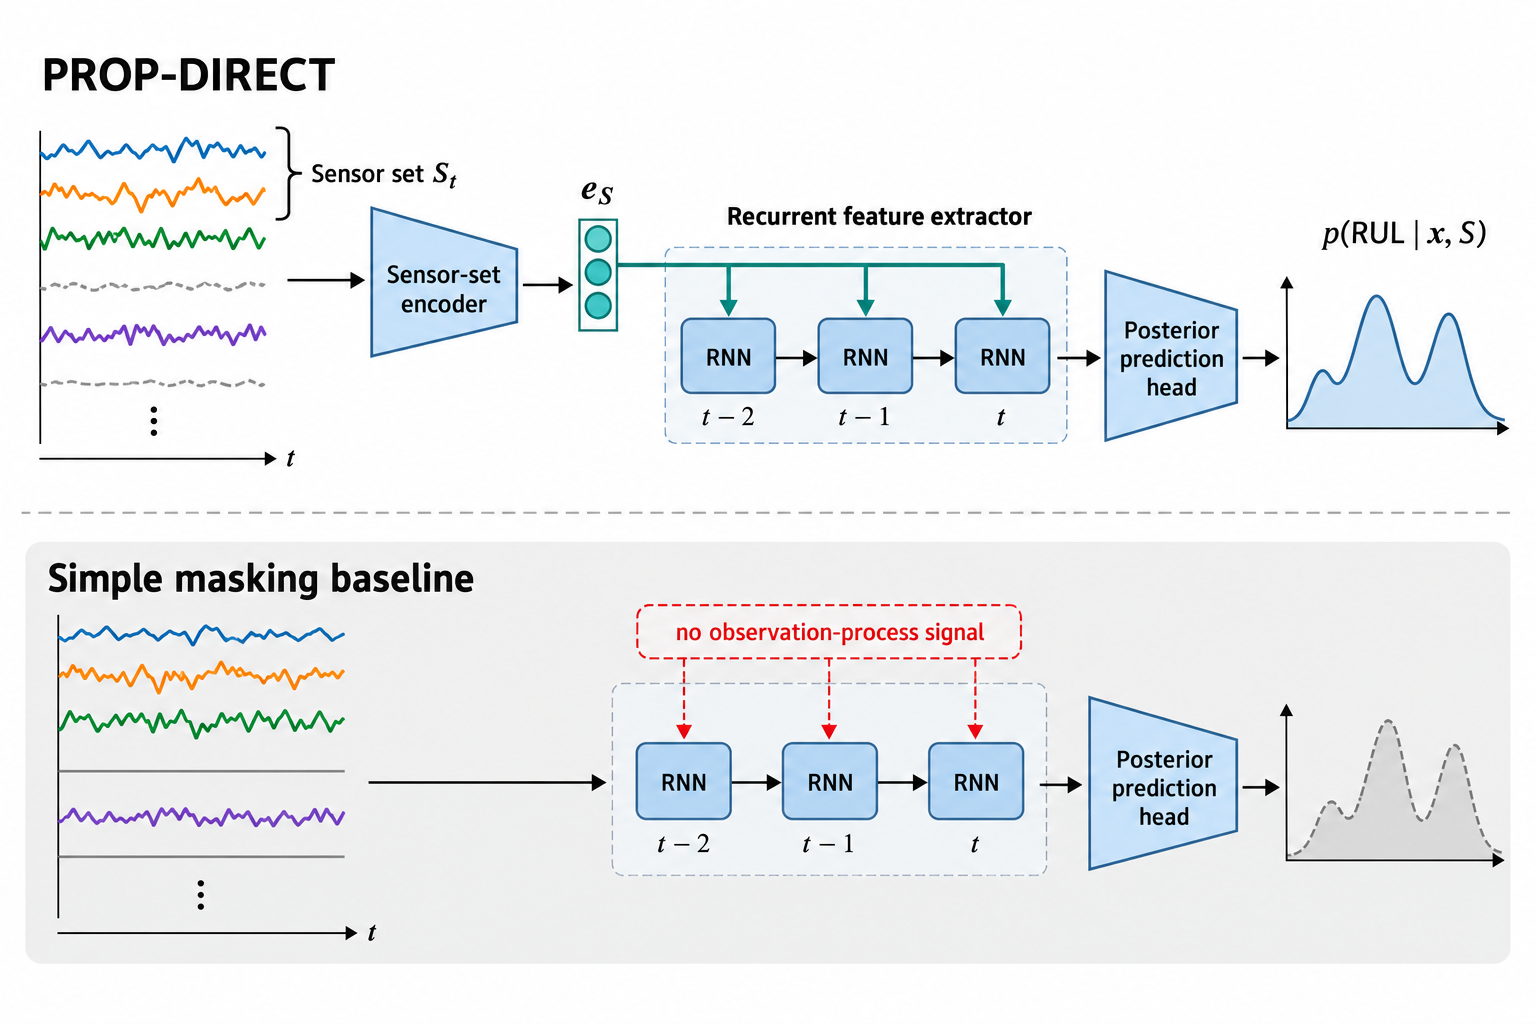
\includegraphics[width=0.86\linewidth]{fig1_prop_direct_architecture.png}
  \caption{\textbf{Observation-process conditioning in PROP-DIRECT.} The model
  encodes the available sensor set as $\mathbf{e}_{\mathcal{S}}$ and injects that
  representation into each recurrent step before predicting the RUL posterior.
  The lower strip shows the masking baseline, which replaces missing values but
  provides no explicit observation-process signal.}
  \label{fig:prop-direct-architecture}
\end{figure}

\paragraph{Sensor-Set Encoder}
Given an observation at time $t$ from asset $a$, let $\mathcal{S}_t$ denote the set of available sensors and $\mathbf{x}_t \in \mathbb{R}^{|\mathcal{S}_t| \times d}$ the observed sensor values over a historical window of length $d$. The sensor-set encoder maps $\mathcal{S}_t$ to a fixed-dimensional embedding $\mathbf{e}_{\mathcal{S}} \in \mathbb{R}^{k}$:
\[
\mathbf{e}_{\mathcal{S}} = f_{\text{enc}}(\mathcal{S}_t; \theta_{\text{enc}})
\]

We implement $f_{\text{enc}}$ as a set encoder using a learned lookup table: each sensor has an embedding vector, and $\mathbf{e}_{\mathcal{S}}$ is computed as the element-wise mean of embeddings for sensors in $\mathcal{S}_t$. This permutation-invariant design ensures the representation does not depend on sensor ordering.

\paragraph{Observation-Conditioned Feature Extraction}
The observed sensor values $\mathbf{x}_t$ are processed by a recurrent encoder (LSTM or GRU) that is \emph{conditioned} on $\mathbf{e}_{\mathcal{S}}$:
\[
\mathbf{h}_t = f_{\text{rnn}}(\mathbf{x}_t, \mathbf{e}_{\mathcal{S}}; \theta_{\text{rnn}})
\]

Conditioning is implemented by concatenating $\mathbf{e}_{\mathcal{S}}$ with the hidden state at each recurrent step, enabling the feature extraction process to adapt based on sensor availability. This differs from standard masking approaches where the recurrent network sees only the values (or masked versions) without explicit knowledge of the observation configuration.

\paragraph{Posterior Prediction Head}
The extracted features $\mathbf{h}_t$ are passed to a prediction head that outputs distributional parameters for the remaining useful life (RUL) posterior. We model RUL as a mixture of log-normal distributions to capture multi-modal degradation behavior:
\[
p(\text{RUL} \mid \mathbf{x}_t, \mathcal{S}_t) = \sum_{i=1}^{M} \pi_i(\mathbf{h}_t, \mathbf{e}_{\mathcal{S}}) \cdot \text{LogNormal}(\mu_i(\mathbf{h}_t, \mathbf{e}_{\mathcal{S}}), \sigma_i(\mathbf{h}_t, \mathbf{e}_{\mathcal{S}}))
\]

Critically, all distributional parameters $\{\pi_i, \mu_i, \sigma_i\}$ depend on \emph{both} the observed data $\mathbf{h}_t$ and the sensor-set embedding $\mathbf{e}_{\mathcal{S}}$. This dual conditioning enables the posterior geometry to explicitly vary with observation configuration.

\subsubsection{Training Objective}

The model is trained to maximize the log-likelihood of observed failure times across diverse sensor configurations:
\[
\mathcal{L} = \sum_{(a,t,\mathcal{S}) \in \mathcal{D}} \log p(\text{RUL}_{a,t} \mid \mathbf{x}_{a,t}, \mathcal{S}; \theta)
\]

where $\mathcal{D}$ is the training dataset covering multiple assets, query times, and sensor configurations. The training data is deliberately constructed to include a variety of observation processes (not just the full sensor complement) so the model learns to adjust posteriors appropriately for different configurations.

\subsection{Baseline Architectures}
\label{sec:methods:baselines}

To isolate the contribution of observation-process conditioning, we compare PROP-DIRECT to six baseline architectures, all trained on the same data and evaluated with the same protocol:

\paragraph{B-STDPROB (Standard Probabilistic Baseline)}
A recurrent neural network with a mixture-of-log-normals output distribution, but \emph{without} sensor-set conditioning. The architecture sees masked inputs (zeros for missing sensors) but does not receive explicit information about which sensors are available. This is the primary comparison model for isolating the effect of conditioning.

\paragraph{B-INDEP (Independent Sensor Baseline)}
Treats each sensor independently without modeling temporal or cross-sensor dependencies. Provides a lower bound on performance.

\paragraph{B-INVAR (Time-Invariant Baseline)}
Uses only static asset features without temporal modeling. Tests whether observation-process conditioning provides value beyond time-invariant prediction.

\paragraph{B-CDE (Conditional Density Estimation)}
A density estimation approach that models $p(\text{RUL} \mid \mathbf{x})$ directly via kernel methods rather than parametric distributions. Provides an alternative uncertainty quantification strategy.

\paragraph{B-SET (Set-Based Aggregation)}
Aggregates sensor values using permutation-invariant pooling (max, mean, attention-weighted) without explicit recurrence. Tests whether set structure alone suffices without temporal modeling.

\paragraph{B-WIDEN (Wider Network)}
A standard architecture (like B-STDPROB) but with increased capacity (more layers, wider hidden states). Controls for the possibility that PROP-DIRECT's gains come from additional parameters rather than conditioning structure.

All models are trained with the same optimization procedure (Adam optimizer, learning rate schedule, early stopping criteria) and hyperparameters are selected via validation set performance to ensure fair comparison.

\subsection{Synthetic Data Generator}
\label{sec:methods:generator}

\subsubsection{Rationale for Synthetic Data}

Rigorous evaluation of observation-process conditioning requires knowing the \emph{true} posterior distribution under different sensor configurations—what we term the ``oracle posterior.'' Real-world PHM datasets do not provide this ground truth, making it impossible to directly measure whether predicted posteriors are geometrically consistent with true posteriors.

We therefore employ a controlled synthetic generator based on established degradation physics. This generator enables:
\begin{itemize}
    \item \textbf{Oracle posterior computation:}\\
    Exact calculation of $p(\RUL \mid \text{observations}, \text{degradation state})$ for any sensor configuration.
    \item \textbf{Causal manipulation:} Controlled variation of observation processes while holding asset state fixed, enabling causal attribution.
    \item \textbf{Importance ground truth:} Explicit specification of which sensors are critical versus redundant, necessary for evaluating importance-awareness.
\end{itemize}

We emphasize that synthetic data limits external validity—findings may not transfer to real industrial assets—but it is essential for the mechanistic analysis conducted here. Section~\ref{sec:limitations} discusses this trade-off in detail.

\subsubsection{Generator Structure}

The generator models asset degradation as a latent Markov process with observable sensor readings:

\paragraph{Degradation Dynamics}
Each asset's health state $\mathbf{z}_t \in \mathbb{R}^{D}$ evolves according to:
\[
\mathbf{z}_{t+1} = g(\mathbf{z}_t, \boldsymbol{\theta}_{\text{phys}}) + \boldsymbol{\epsilon}_t, \quad \boldsymbol{\epsilon}_t \sim \mathcal{N}(0, \Sigma_{\text{proc}})
\]

where $g(\cdot)$ is a physics-based degradation function (e.g., exponential bearing wear, cumulative fatigue damage) parameterized by $\boldsymbol{\theta}_{\text{phys}}$, and $\boldsymbol{\epsilon}_t$ represents process noise. The asset fails when any component of $\mathbf{z}_t$ crosses a failure threshold, defining the true RUL.

\paragraph{Observation Process}
Sensor readings $\mathbf{x}_t$ are noisy functions of the latent state:
\[
x_{s,t} = h_s(\mathbf{z}_t) + \eta_{s,t}, \quad \eta_{s,t} \sim \mathcal{N}(0, \sigma_s^2)
\]

where $h_s(\cdot)$ maps latent health to sensor $s$'s measurement and $\eta_{s,t}$ is observation noise. Different sensors have different mappings $h_s$:
\begin{itemize}
    \item \textbf{Critical sensors} directly observe components near failure thresholds (e.g., vibration monitoring bearing wear).
    \item \textbf{Redundant sensors} observe the same physical quantity with independent noise (e.g., multiple temperature probes on the same subsystem).
    \item \textbf{Ancillary sensors} observe tangentially related quantities (e.g., ambient temperature when bearing temperature is critical).
\end{itemize}

\paragraph{Observation Configurations}
The generator samples sensor availability configurations according to specified distributions:
\begin{itemize}
    \item \textbf{Full configuration:} All sensors available (baseline).
    \item \textbf{Sufficient deletions:} Remove ancillary or redundant sensors, maintaining critical coverage.
    \item \textbf{Critical deletions:} Remove sensors that directly observe near-failure states.
    \item \textbf{Random deletions:} Remove sensors uniformly at random, matched in count to critical deletions.
\end{itemize}

The causal structure of this generator is shown in Figure~\ref{fig:synthetic-generator}.
It separates the latent degradation state from noisy measurements and makes the
critical, redundant, and ancillary sensor roles explicit.

\begin{figure}[!ht]
  \centering
  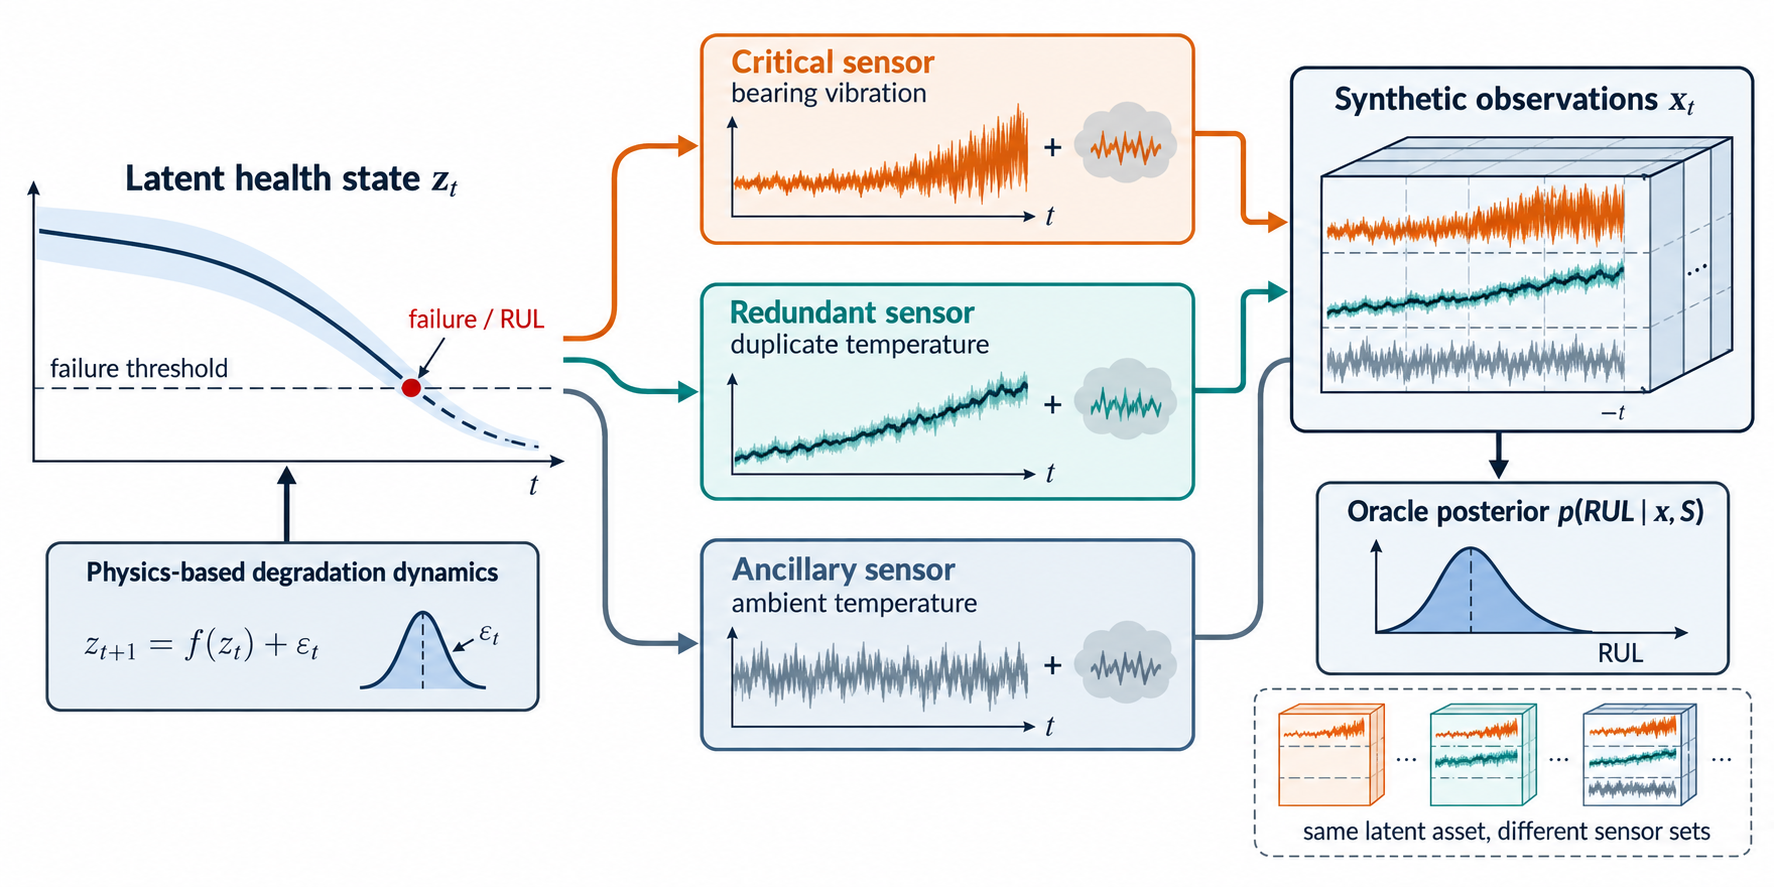
\includegraphics[width=0.86\linewidth]{fig4_synthetic_generator.png}
  \caption{\textbf{Synthetic degradation-data generator.} A latent health state
  evolves under physics-based dynamics and crosses a failure threshold at the
  true RUL. Noisy observation channels produce critical, redundant, and ancillary
  sensors, while different sensor subsets of the same latent asset support exact
  oracle-posterior computation.}
  \label{fig:synthetic-generator}
\end{figure}
\FloatBarrier

\subsubsection{Asset Population}

We generate 96 synthetic assets with the following variation:
\begin{itemize}
    \item \textbf{Degradation parameters} $\boldsymbol{\theta}_{\text{phys}}$: Sampled to produce heterogeneous failure times (mean RUL: 5000 cycles, range: 2000–8000).
    \item \textbf{Observation noise} $\sigma_s^2$: Varies across sensors and assets to simulate sensor quality differences.
    \item \textbf{Operating conditions:} Three regimes (low/medium/high load) affecting degradation rates.
    \item \textbf{Sensor topologies:} Different mappings $h_s(\cdot)$ to simulate domain variety (e.g., vibration-dominated vs. temperature-dominated degradation).
\end{itemize}

Each asset is observed from initial deployment until failure, with queries sampled at regular intervals (every 50 cycles) throughout its lifecycle. This produces approximately 96 assets $\times$ 100 query times $\times$ multiple observation configurations = tens of thousands of evaluation cases.

\subsection{Study Design and Evaluation Protocol}
\label{sec:methods:protocol}

\subsubsection{Preregistration and Data Partitioning}

To ensure statistical integrity, we employ a preregistered evaluation protocol where all decision criteria, thresholds, and analysis plans are specified \emph{before} accessing evaluation outcomes. The protocol proceeds in stages:

Figure~\ref{fig:preregistration-protocol} provides a compact view of the four
stages and the separation between exploratory development, test replication, and
the lockbox used for the primary claim.

\begin{figure}[!ht]
  \centering
  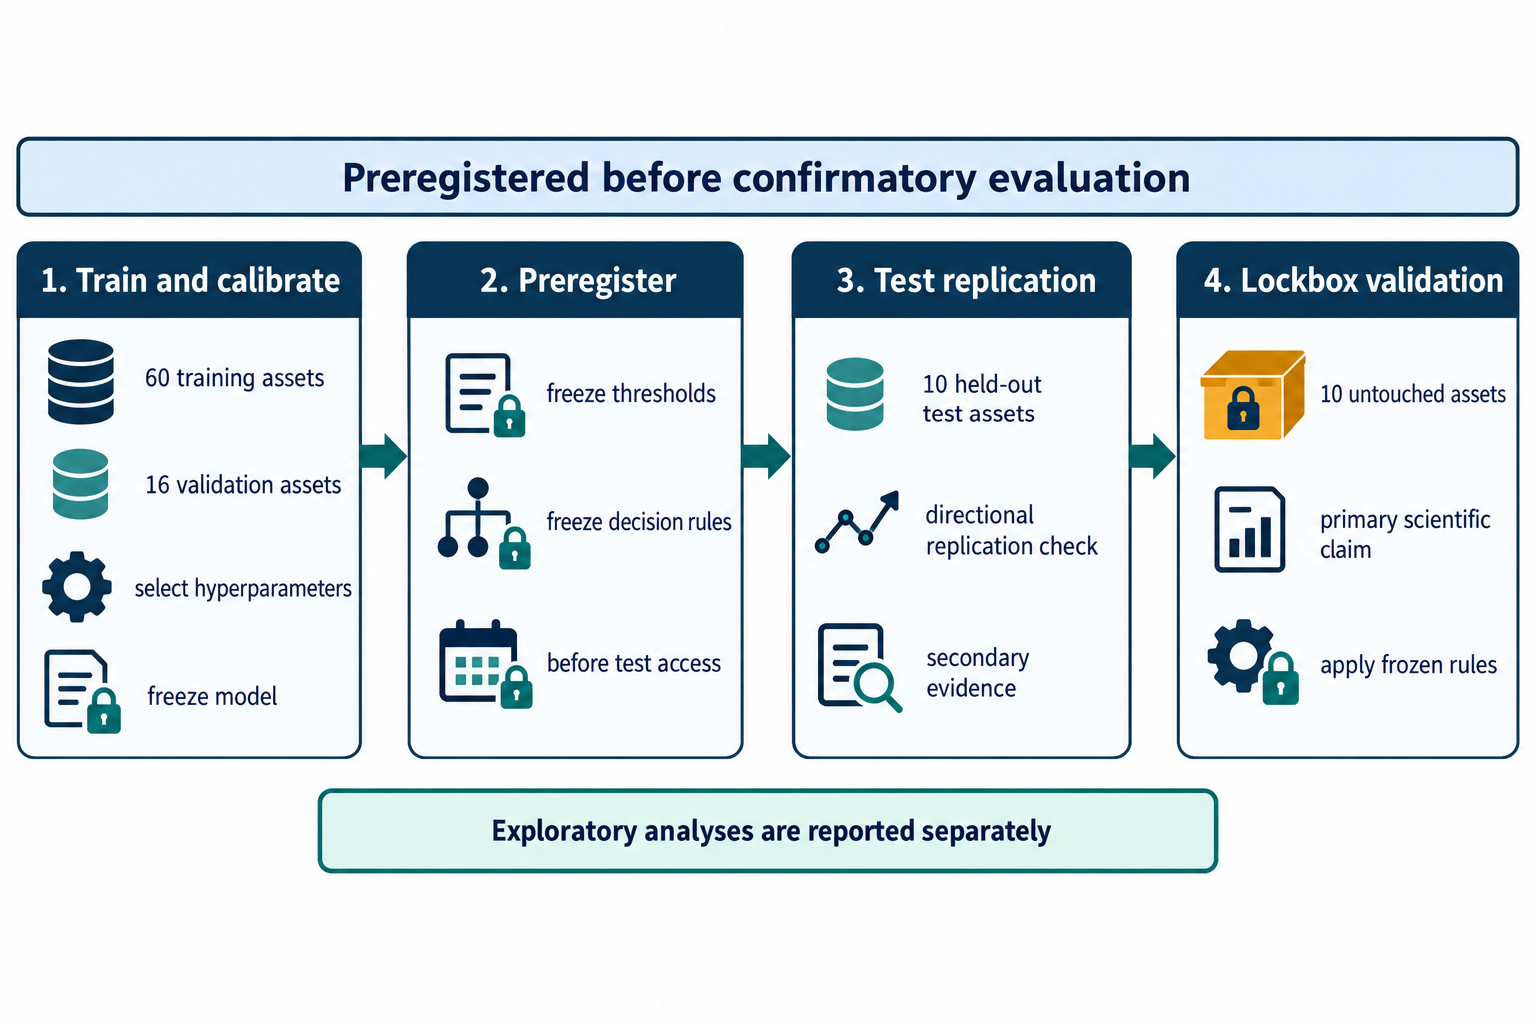
\includegraphics[width=0.86\linewidth]{fig5_preregistration_protocol.png}
  \caption{\textbf{Preregistered evaluation protocol.} Model development and
  threshold selection are completed before held-out evaluation. The test split
  serves as a directional replication check, whereas the untouched lockbox is
  evaluated with frozen decision rules and supplies the primary scientific claim.}
  \label{fig:preregistration-protocol}
\end{figure}
\FloatBarrier

\paragraph{Stage 1: Model Development and Freezing}
\begin{enumerate}
    \item Train all seven models (PROP-DIRECT + six baselines) on a designated training set (60 assets).
    \item Select hyperparameters via validation set performance (16 assets).
    \item Freeze model checkpoints and record them in a versioned registry.
\end{enumerate}

\paragraph{Stage 2: Threshold Specification}
\begin{enumerate}
    \item Using the validation set and power analysis, specify:
    \begin{itemize}
        \item Non-inferiority margins for quality metrics (MAE, CRPS).
        \item Superiority margins for geometric consistency metrics.
        \item Acceptability thresholds for absolute geometry.
    \end{itemize}
    \item Commit these thresholds to a frozen registry before scoring test or lockbox data.
\end{enumerate}

\paragraph{Stage 3: Test Split Evaluation}
\begin{enumerate}
    \item Score all models on a held-out test split (10 assets) using frozen checkpoints.
    \item Compare outcomes to preregistered criteria.
    \item This stage serves as a ``replication check''—we expect consistent direction of effects with the validation set but do not make final scientific claims based on test results alone.
\end{enumerate}

\paragraph{Stage 4: Lockbox Validation}
\begin{enumerate}
    \item Score all models on a fully held-out lockbox split (10 assets) that no human has inspected during development.
    \item Apply preregistered decision rules to lockbox outcomes.
    \item Lockbox results are the primary basis for scientific claims.
\end{enumerate}

This staging records which decisions are made before each held-out evaluation and keeps exploratory analyses separate from the primary claim.

\subsubsection{Data Split Composition}

\begin{itemize}
    \item \textbf{Training:} 60 assets, diverse degradation parameters and sensor configurations.
    \item \textbf{Validation:} 16 assets, used for hyperparameter selection and threshold calibration.
    \item \textbf{Test:} 10 assets, first held-out evaluation for replication check.
    \item \textbf{Lockbox:} 10 assets, fully independent validation for primary claims.
\end{itemize}

All splits are stratified by degradation regime (low/medium/high load) and sensor topology to ensure balanced representation.

The partition above applies to the sufficient-observation analysis, whose primary claims rest on the lockbox split. The information-loss analysis uses a separate frozen evaluation covering all 96 assets; its descriptive quality metrics (Table~\ref{tab:c2_quality}) therefore summarize that population rather than the 10-asset test split. Model checkpoints and decision rules were frozen before either evaluation was accessed.

\subsubsection{Information-loss boundary design}

The boundary analysis compares sensor deletions that differ in functional importance
while holding the number of removed channels fixed. We use three pair classes:
\begin{itemize}
    \item \textbf{Critical deletion:} sensors identified by the oracle analysis as critical for RUL prediction;
    \item \textbf{Random deletion:} the same number of sensors selected at random, providing a matched control for information quantity;
    \item \textbf{Redundant deletion:} sensors carrying overlapping information, providing a low-impact comparison.
\end{itemize}

The corresponding estimand asks whether an importance-aware architecture keeps the
critical-versus-random posterior contrast closer to the oracle-defined contrast than
a model that only observes masked values. This design separates the effect of how
many sensors are removed from the effect of which sensors are removed.

\subsection{Evaluation Metrics}
\label{sec:methods:metrics}

\subsubsection{Geometric Consistency Metrics}

The primary evaluation question is whether PROP-DIRECT produces geometrically consistent posteriors across observation views of the same asset. We measure this via the \emph{cross-view posterior inconsistency} metric:

\paragraph{Paired Observation Setup}
For each asset $a$ at query time $t$, we generate predictions under two observation configurations $\mathcal{S}_1$ and $\mathcal{S}_2$ that should provide compatible information (e.g., full sensors vs. ancillary sensors removed). Denote the predicted posteriors as $p_1 = p(\text{RUL} \mid \mathbf{x}_{a,t}, \mathcal{S}_1)$ and $p_2 = p(\text{RUL} \mid \mathbf{x}_{a,t}, \mathcal{S}_2)$.

\paragraph{Energy Distance}
We quantify inconsistency using the energy distance, a proper metric on probability distributions:
\[
d_E(p_1, p_2) = 2 \mathbb{E}_{Y_1 \sim p_1, Y_2 \sim p_2}[|Y_1 - Y_2|] - \mathbb{E}_{Y_1, Y_1' \sim p_1}[|Y_1 - Y_1'|] - \mathbb{E}_{Y_2, Y_2' \sim p_2}[|Y_2 - Y_2'|]
\]

This metric:
\begin{itemize}
    \item Equals zero if and only if $p_1 = p_2$ (distributional consistency across views).
    \item Increases with both location shift and shape differences.
    \item Does not require parametric assumptions about posterior forms.
\end{itemize}

A small $d_E$ is a consistency statement, not an accuracy statement: a model
that emits the same posterior for every sensor set can attain $d_E=0$ while
ignoring the observation process. To evaluate whether the distance has the
right magnitude, we therefore report the secondary oracle-relative geometry
error
\[
E_{\mathrm{geometry}} = \left|d_E(p_{\mathrm{model},1},p_{\mathrm{model},2}) - d_E(p_{\mathrm{oracle},1},p_{\mathrm{oracle},2})\right|.
\]
Lower values indicate closer agreement with the oracle-defined geometry. This
post-hoc quantity is reported as an exploratory diagnostic and does not replace
the preregistered cross-view consistency endpoint.

In practice, we estimate $d_E$ via Monte Carlo sampling: draw $N=256$ samples from each posterior (or $N=64$ for computational budget sensitivity), compute pairwise distances, and average.

\paragraph{Metric Scale and Interpretation}
All metrics (energy distance, MAE, CRPS) are computed on \emph{normalized RUL values}. Normalization is performed by dividing each asset's RUL by its maximum observed lifetime. For the synthetic generator used here, the mean lifetime is 5000 cycles (range: 2000--8000), so an energy distance of $2.86 \times 10^{-4}$ in normalized units corresponds to approximately 1.4 cycles of absolute distribution separation when scaled back to the raw RUL scale. Similarly, a normalized MAE of 0.015 corresponds to approximately 75 cycles of prediction error at mean scale.

This normalization ensures metrics are comparable across assets with heterogeneous lifetimes and enables threshold specification in scale-invariant units. All thresholds ($\tau$ for superiority margins, acceptability bounds for absolute geometry) are specified in these normalized units and frozen prior to evaluation.

\paragraph{Off-Diagonal Correction}
To avoid spurious correlation from comparing a sample to itself, we use an off-diagonal estimator: when computing cross-distribution expectations $\mathbb{E}_{Y_1, Y_2}[|Y_1 - Y_2|]$, we exclude pairs where the same random number stream was used. This correction is critical for the mechanistic analysis where sample efficiency matters.

\paragraph{Aggregation}
For each model and observation-process pair type (e.g., full vs. ancillary-removed), we compute:
\begin{enumerate}
    \item Asset-level geometry: Mean energy distance over all query times for that asset.
    \item Population-level geometry: Mean over all assets.
\end{enumerate}

The primary estimand is the \emph{relative reduction}:
\[
\text{Relative reduction} = \frac{d_E(\text{B-INDEP}) - d_E(\text{PROP-DIRECT})}{d_E(\text{B-INDEP})} \times 100\%
\]

where B-INDEP serves as the observation-agnostic baseline. A positive value indicates PROP-DIRECT is more consistent.

\paragraph{Baseline Selection}
B-INDEP is the preregistered primary comparator because it treats sensor
channels independently and provides an observation-agnostic reference. We also
report B-STDPROB, which shares the observation interface of PROP-DIRECT. Their
near-identical energy distances on the test and lockbox splits
(Table~\ref{tab:baseline_comparison}) provide a complementary baseline check.

\subsubsection{Quality Metrics}

To verify that geometric improvements do not come at the cost of prediction quality, we evaluate:

\paragraph{Mean Absolute Error (MAE)}
For RUL point predictions (posterior median):
\[
\text{MAE} = \frac{1}{N} \sum_{i=1}^{N} |\text{RUL}_{\text{true},i} - \text{RUL}_{\text{pred},i}|
\]

Computed separately for all time points (state MAE) and time points within 500 cycles of failure (failure MAE), as accuracy near failure is often more operationally critical.

\paragraph{Continuous Ranked Probability Score (CRPS)}
A proper scoring rule for probabilistic forecasts:
\[
\text{CRPS}(p, y) = \mathbb{E}_{Y \sim p}[|Y - y|] - \frac{1}{2} \mathbb{E}_{Y, Y' \sim p}[|Y - Y'|]
\]

where $p$ is the predicted distribution and $y$ is the observed RUL. CRPS jointly evaluates calibration (whether prediction intervals cover the true value at nominal rates) and sharpness (whether intervals are tight). Lower CRPS indicates better probabilistic prediction.

\paragraph{Calibration diagnostics}
As a complementary descriptive check, we compute central-interval coverage at nominal levels of 50\%, 80\%, and 90\% from the persisted posterior samples. We also compute the probability integral transform (PIT) for each coordinate using the mid-rank of the observed target among the predictive samples. Coverage is summarized over the three coordinates, while PIT histograms are compared with the uniform benchmark. These diagnostics are evaluated after the preregistered scoring and do not change any decision threshold or model designation.

\subsubsection{Statistical Inference}

\paragraph{Bootstrap Confidence Intervals}
All primary estimates are accompanied by 90\% bootstrap confidence intervals computed as follows:
\begin{enumerate}
    \item Resample assets with replacement (preserving within-asset dependencies).
    \item Recompute the estimand (e.g., relative reduction) on the resampled data.
    \item Repeat 2,000 times.
    \item Report the 5th and 95th percentiles of the bootstrap distribution.
\end{enumerate}

\paragraph{Decision Rules}
Preregistered decision criteria:
\begin{itemize}
    \item \textbf{Superiority claim:} The 90\% CI must exclude zero \emph{and} exclude a prespecified margin $\tau$ representing the minimum scientifically meaningful effect.
    \item \textbf{Non-inferiority claim:} The 90\% CI lower bound must exceed a non-inferiority margin (e.g., $-\tau$).
    \item \textbf{Quality guardrails:} CRPS and MAE must satisfy non-inferiority vs. baseline to ensure geometric gains do not degrade prediction quality.
\end{itemize}

\subsection{C-MAPSS Shared-Model Evaluation}
\label{sec:methods:cmapss}

We use C-MAPSS FD001 as a complementary public simulated benchmark. The dataset
contains 100 training and 100 test engine trajectories and 14 non-constant sensor
channels after preprocessing. It provides a common reference for the geometry
analysis while remaining distinct from field data.

We retain the full 14-channel view and construct two reduced views by deleting
three channels from each; the deletion sets differ by six channels. For each method,
a single predictor is trained on the union of all three views. The 100 training
engines are split by engine into 80 fitting and 20 validation engines, so views of
the same engine never cross a split. Unlike the synthetic experiments, which use an
explicitly distributional mixture-of-log-normals head, C-MAPSS uses an MSE
point-prediction head. We construct predictive samples with 128 Monte Carlo dropout
passes~\citep{gal2016dropout}. This is a complementary uncertainty representation,
not a direct replication of the synthetic posterior model. We evaluate the final
window of each test engine, report energy distances on the raw RUL scale, and use
engine-level bootstrap resampling for confidence intervals. Single-view MAE is
reported as a point-accuracy check alongside the geometry results.

This protocol tests whether the geometry pattern survives a shared-model training
setup. Because the benchmark is simulated and the reduced views are created by
artificial deletion, its results are interpreted as complementary benchmark evidence
rather than field validation.

\subsection{Exploratory Mechanistic Analysis}
\label{sec:methods:exploratory}

Beyond the preregistered analysis, we use an exploratory oracle comparison to interpret the different regimes. It is hypothesis-generating rather than a confirmatory test.

\paragraph{Oracle-Model Correlation}
For each paired observation case, we compute:
\begin{itemize}
    \item \textbf{Oracle distance:} The true geometric inconsistency $d_E(p_{\text{oracle},1}, p_{\text{oracle},2})$ computed from the known ground-truth degradation state.
    \item \textbf{Oracle-relative geometry error:} The residual
    $E_{\mathrm{geometry}}=|d_E(p_{\text{model},1},p_{\text{model},2})-d_E(p_{\text{oracle},1},p_{\text{oracle},2})|$.
\end{itemize}

If the model successfully tracks task difficulty, these should correlate: cases where the oracle shows large inconsistency (observation processes genuinely differ) should also exhibit large model inconsistency.

We compute Pearson correlation $r$ separately for different observation-process pair types (critical vs. full, critical vs. random, etc.). Because prediction cases share assets and query structure, the correlations describe an effect-size pattern rather than a confirmatory independent-sample test. Asset-level or mixed-effects inference is a natural follow-up.

\subsection{Computational Environment}

All experiments are conducted on NVIDIA A40 GPUs with 48GB memory. Model training uses mixed-precision (FP16) arithmetic via PyTorch's automatic mixed precision. Evaluation scoring uses full FP32 precision to ensure numerical stability in bootstrap resampling. Monte Carlo sampling for energy distance computation is parallelized across query times and assets. Total computational budget: approximately 500 GPU-hours for training all models, 100 GPU-hours for evaluation scoring across all splits and configurations.

Code and model checkpoints are archived with version control (Git) to enable
exact replication. The complete evaluation pipeline, including bootstrap
resampling and decision logic, is frozen prior to lockbox evaluation and
committed to the archive.

% Revised Results - Publication Quality
% Clear narrative structure with meaningful section names

\section{Results}
\label{sec:results}

We first report the primary cross-view result under task-sufficient observation. We then locate its boundary under critical sensor loss, interpret that boundary with an exploratory oracle comparison, and separate geometric behavior from predictive quality and calibration. The section closes with a complementary shared-model evaluation on C-MAPSS. Unless stated otherwise, intervals in the synthetic analyses use 2,000 asset-level bootstrap replicates.

\subsection{Cross-View Consistency Under Sufficient Observation}
\label{sec:results:sufficient}

\subsubsection{Primary Finding}

When observation processes maintain task sufficiency---that is, when different sensor subsets all support reliable RUL prediction---PROP-DIRECT substantially reduces posterior inconsistency across views of the same asset. Table~\ref{tab:c1_resolution} reports the formal lockbox validation results.

\begin{table}[tb]
  \centering
  \caption{Resolution sensitivity on the lockbox split. Intervals are
  two-sided 90\% bootstrap confidence intervals with 2,000 replicates.}
  \label{tab:c1_resolution}
  \begin{tabular}{lccc}
    \toprule
    Sampling budget & PROP-DIRECT geometry & Relative reduction & 90\% CI \\
    \midrule
    256 (primary) & 0.0002864 & 38.64\% & [34.78\%, 42.44\%] \\
    64 (check)    & 0.0002849 & 38.97\% & [35.03\%, 42.66\%] \\
    \bottomrule
  \end{tabular}
\end{table}

% Table: Baseline Consistency Comparison
% Addresses P0-2: Shows improvement is robust across baseline choices

\begin{table}[t]
\centering
\begin{threeparttable}
\caption{\textbf{Geometric consistency comparison across baselines.}
Energy distance for PROP-DIRECT and two observation-agnostic baselines
under the sufficient observation regime. Relative reduction computed as
$(d_E(\text{baseline}) - d_E(\text{PROP})) / d_E(\text{baseline}) \times 100\%$.
Lower energy distance indicates better cross-view posterior consistency.
Both baselines yield comparable absolute energy distance, confirming
that relative improvements are robust to baseline choice.}
\label{tab:baseline_comparison}
\begin{tabular}{llcc}
\toprule
\textbf{Split} & \textbf{Model} & \textbf{Energy Distance} & \textbf{Relative Reduction} \\
\midrule
Test   & PROP-DIRECT  & $2.89 \times 10^{-4}$ & --- \\
       & B-STDPROB    & $4.57 \times 10^{-4}$ & 36.8\% \\
       & B-INDEP      & $4.66 \times 10^{-4}$ & 38.0\% \\
\midrule
Lockbox & PROP-DIRECT  & $2.86 \times 10^{-4}$ & --- \\
        & B-STDPROB    & $4.64 \times 10^{-4}$ & 38.3\% \\
        & B-INDEP      & $4.67 \times 10^{-4}$ & 38.6\% \\
\bottomrule
\end{tabular}
\begin{tablenotes}
\footnotesize
\item Bootstrap 90\% confidence intervals for the primary comparison
(PROP-DIRECT vs B-INDEP): Test [35.1\%, 40.7\%], Lockbox [34.8\%, 42.4\%].
B-STDPROB and B-INDEP differ by less than 1\% in absolute energy distance,
indicating that the choice of observation-agnostic baseline does not
materially affect conclusions.
\end{tablenotes}
\end{threeparttable}
\end{table}


The architecture achieves an absolute geometry metric of $2.86 \times 10^{-4}$ on the lockbox split, well below the pre-specified acceptability threshold of $3.5 \times 10^{-4}$. More importantly, this represents a \textbf{38.6\% reduction} (90\% CI: 34.8--42.4\%) in cross-view inconsistency relative to the observation-agnostic baseline (B-INDEP). The test split yields a consistent 38.1\% reduction (90\% CI: 34.2--41.9\%), confirming the effect is not an artifact of a single data partition.

Because a small cross-view distance can also result from an invariant predictor, we
additionally inspected the frozen oracle-relative quantity defined in
Section~\ref{sec:methods:metrics}. On the lockbox split, the asset-level mean
$E_{\mathrm{geometry}}$ was $8.07\times10^{-4}$ for PROP-DIRECT and
$9.29\times10^{-4}$ for B-STDPROB; the corresponding test values were
$6.89\times10^{-4}$ and $7.96\times10^{-4}$. These are descriptive post-hoc
summaries, not a replacement for the preregistered consistency endpoint; the
asset-bootstrap comparison for the information-loss regimes is reported later in
Table~\ref{tab:oracle_alignment}.

Figure~\ref{fig:c1-forest} visualizes the same effect sizes and confidence
intervals. The close alignment of the test and lockbox estimates makes the
replication pattern visible without relying on a numerical comparison alone.

\begin{figure}[!ht]
  \centering
  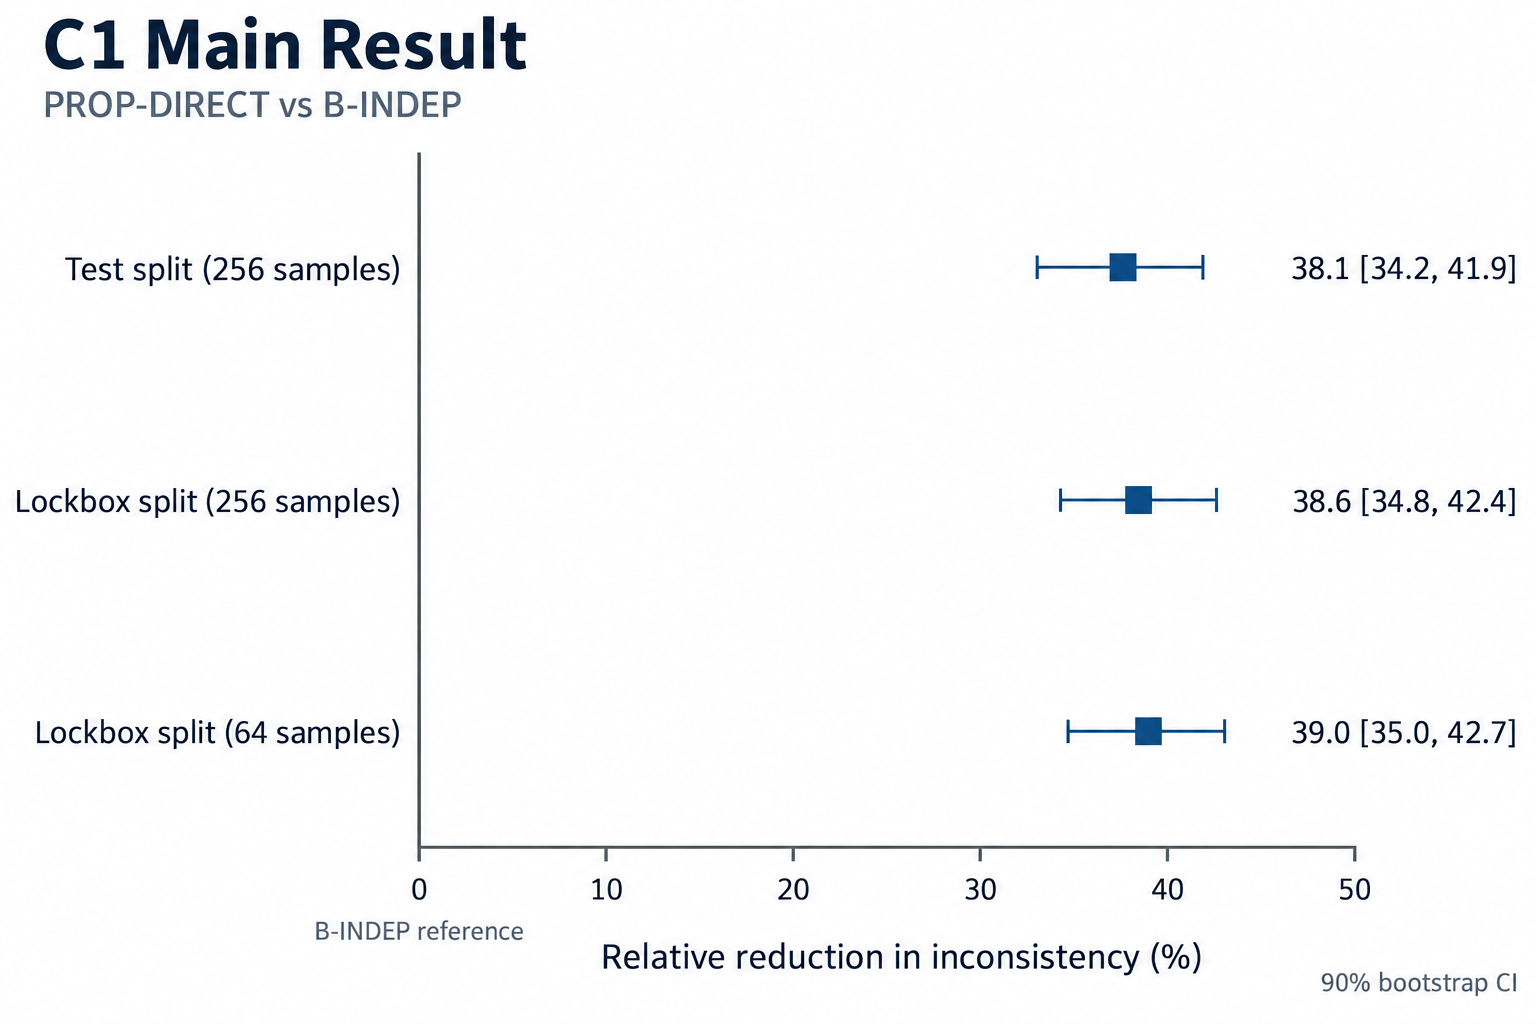
\includegraphics[width=0.86\linewidth]{fig2_c1_main_result_forest.png}
  \caption{\textbf{Primary consistency result.} PROP-DIRECT reduces cross-view posterior
  inconsistency relative to B-INDEP by approximately 38\% on both the test and
  lockbox splits. Squares show point estimates and horizontal bars show 90\%
  bootstrap confidence intervals; the reduced 64-sample budget produces the same
  conclusion.}
  \label{fig:c1-forest}
\end{figure}

Predictions from different views of the same asset are therefore substantially closer in posterior geometry. The result motivates testing whether such alignment improves uncertainty-aware maintenance decisions, where prediction intervals and tail probabilities influence action.

\subsubsection{Robustness to Sampling Budget}

A critical deployment consideration is computational cost. Uncertainty quantification via Monte Carlo sampling typically dominates inference time, making sampling budget a key engineering constraint. We therefore evaluated whether the geometric improvement persists under reduced sampling.

When the Monte Carlo budget is reduced four-fold from 256 to 64 samples per prediction, the effect size changes by only 0.34 percentage points: 38.97\% reduction (90\% CI: 35.03--42.67\%) versus 38.64\% at the standard budget. This stability indicates that the geometric benefit does not rely on high-precision uncertainty estimation within the synthetic evaluation; whether this translates into an acceptable deployment latency trade-off requires a direct systems benchmark.

\subsubsection{Interpretation}

These results support the hypothesis that explicit observation-process conditioning enables models to align posterior geometry across compatible views. The architecture appears to learn that different sensor configurations, when task-sufficient, should produce posteriors that overlap appropriately rather than diverging arbitrarily. The robustness to sampling budget suggests this is a structural property of the learned representations, not a fragile artifact of estimation precision.

\subsection{Boundary Behavior Under Critical Sensor Loss}
\label{sec:results:boundary}

The boundary comparison defined in Section~\ref{sec:methods:protocol} holds the
number of deleted sensors fixed while changing their functional role. It asks
whether the conditioning pathway distinguishes a critical deletion from a matched
random deletion, rather than merely responding to the amount of missing data.

\subsubsection{The Importance Boundary}

PROP-DIRECT does \emph{not} outperform the baseline in this regime. Across three pre-registered estimands measuring different aspects of geometric inconsistency under information loss, all comparisons favor the baseline or show no advantage:

\begin{itemize}
    \item \textbf{Critical-sensor excess risk:} $\Delta R_{\text{crit}} = +8.65 \times 10^{-4}$ (90\% CI: 7.36--9.91 $\times 10^{-4}$)
    \item \textbf{Loss-geometry differential:} $\Delta G_{\text{loss}} = +1.88 \times 10^{-4}$ (90\% CI: $-3.55$ to $+6.99 \times 10^{-4}$)
    \item \textbf{Interaction effect:} $I_R = +7.68 \times 10^{-4}$ (90\% CI: 5.16--10.28 $\times 10^{-4}$)
\end{itemize}

All point estimates are positive, indicating PROP-DIRECT exhibits \emph{greater} inconsistency than the baseline under importance-dependent information loss. The confidence intervals either exclude zero or barely overlap it, providing consistent evidence against the superiority hypothesis.

\subsubsection{Predictive-quality guardrail}

The geometric degradation is accompanied by only a small change in predictive quality. A pre-specified guardrail based on continuous ranked probability score (CRPS)---a proper scoring rule for probabilistic forecasts---gives: $\Delta \text{CRPS} = +4.07 \times 10^{-4}$ (90\% CI: $-0.22$ to $+8.47 \times 10^{-4}$), well below the non-inferiority margin of $3.85 \times 10^{-3}$.

The two metrics therefore capture different aspects of the model: the limitation concerns \emph{geometric consistency}, while single-view RUL prediction remains competitive.

\subsubsection{Pair-Class Decomposition}

Examining the three comparison types reveals structure in the failure:

Figure~\ref{fig:c2-pairs} provides a visual summary of the pair-class ordering
before the numerical decomposition below.

\begin{figure}[!ht]
  \centering
  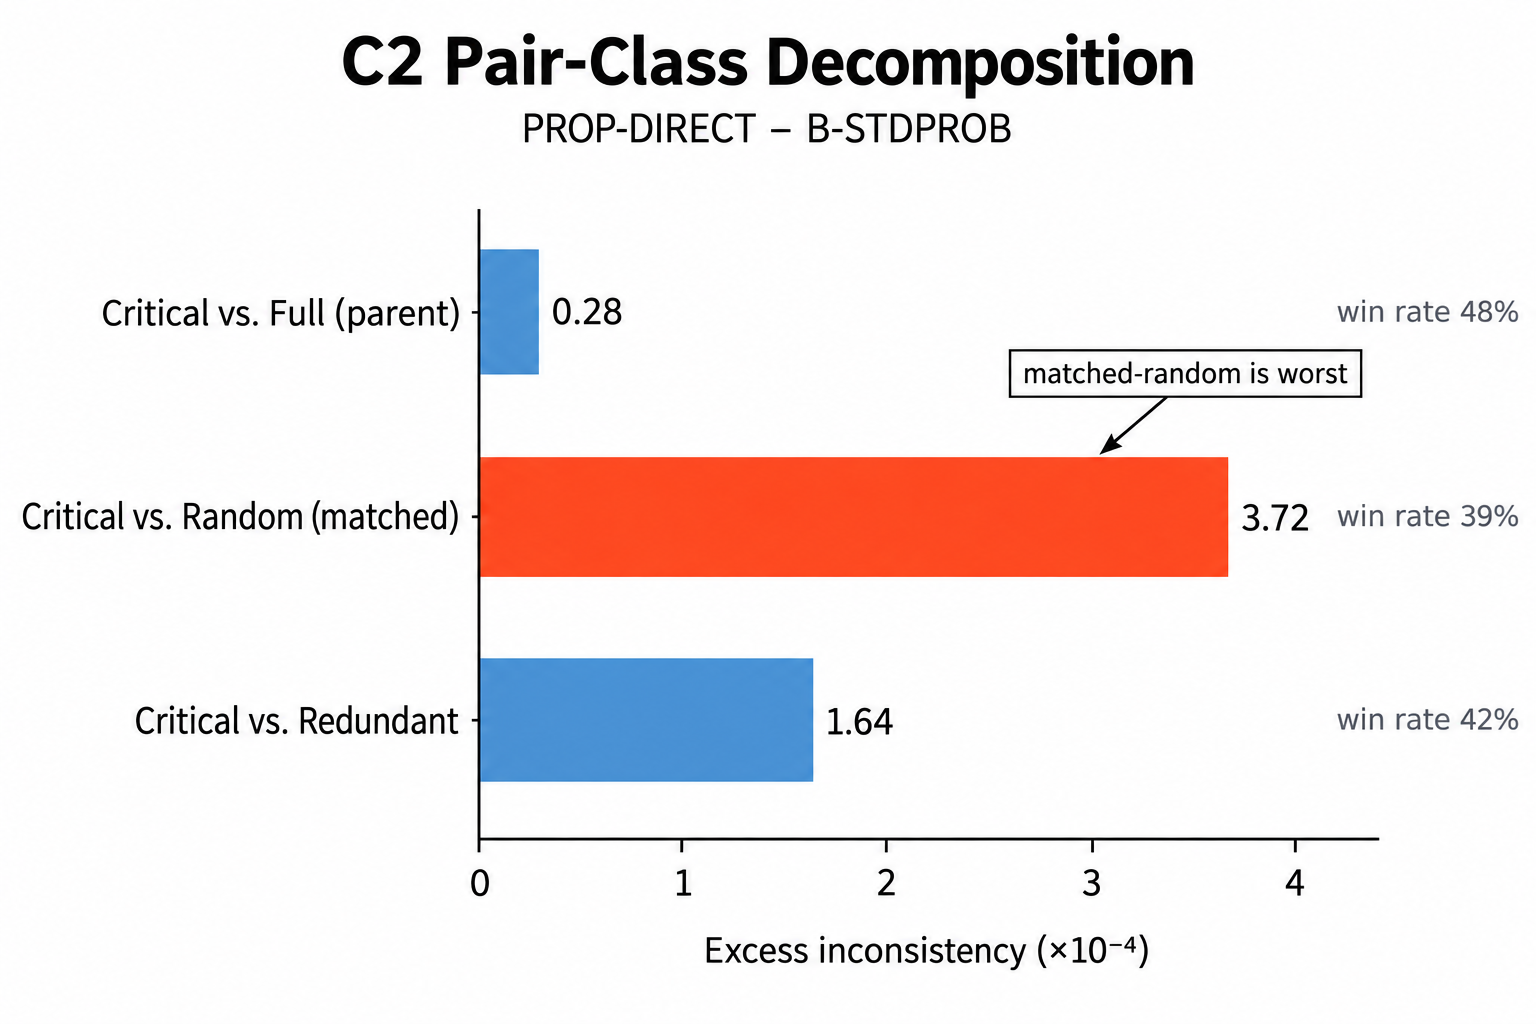
\includegraphics[width=0.75\linewidth]{fig3_c2_pair_class_decomposition.png}
  \caption{\textbf{Information-loss pair-class decomposition.} Excess inconsistency relative
  to B-STDPROB is small for critical-versus-full comparisons but substantially
  larger for the matched-random class. The associated win rates show the same
  ordering, highlighting the pair class in which the current flat sensor-set
  representation is least effective.}
  \label{fig:c2-pairs}
\end{figure}

\begin{center}
\begin{tabular}{lcc}
\toprule
Comparison & Mean Difference & PROP-DIRECT Win Rate \\
\midrule
Critical vs. Full (parent) & $+2.8 \times 10^{-5}$ & 48\% \\
Critical vs. Random (matched) & $+3.72 \times 10^{-4}$ & 39\% \\
Critical vs. Redundant & $+1.64 \times 10^{-4}$ & 42\% \\
\bottomrule
\end{tabular}
\end{center}

The pair-class ordering is informative: PROP-DIRECT is nearly at parity with the
baseline for critical deletion versus the full sensor complement ($+2.8 \times
10^{-5}$ mean difference; 48\% win rate), whereas its excess inconsistency is
larger for random and redundant deletions. The matched-random comparison carries
the largest excess inconsistency and the lowest win rate, making it the clearest
stress test of whether sensor identity, rather than sensor count alone, is
represented.

Figure~\ref{fig:c2-pairs} makes this asymmetry explicit: the matched-random
comparison has the largest excess inconsistency and the lowest PROP-DIRECT win
rate, supporting the interpretation that the architecture detects missing
information more readily than functional sensor importance.

Figure~\ref{fig:prediction-example} makes this contrast concrete for one asset at
one query time: removing ancillary sensors leaves the posterior nearly unchanged,
whereas removing a critical sensor widens and shifts the distribution.

\begin{figure}[!ht]
  \centering
  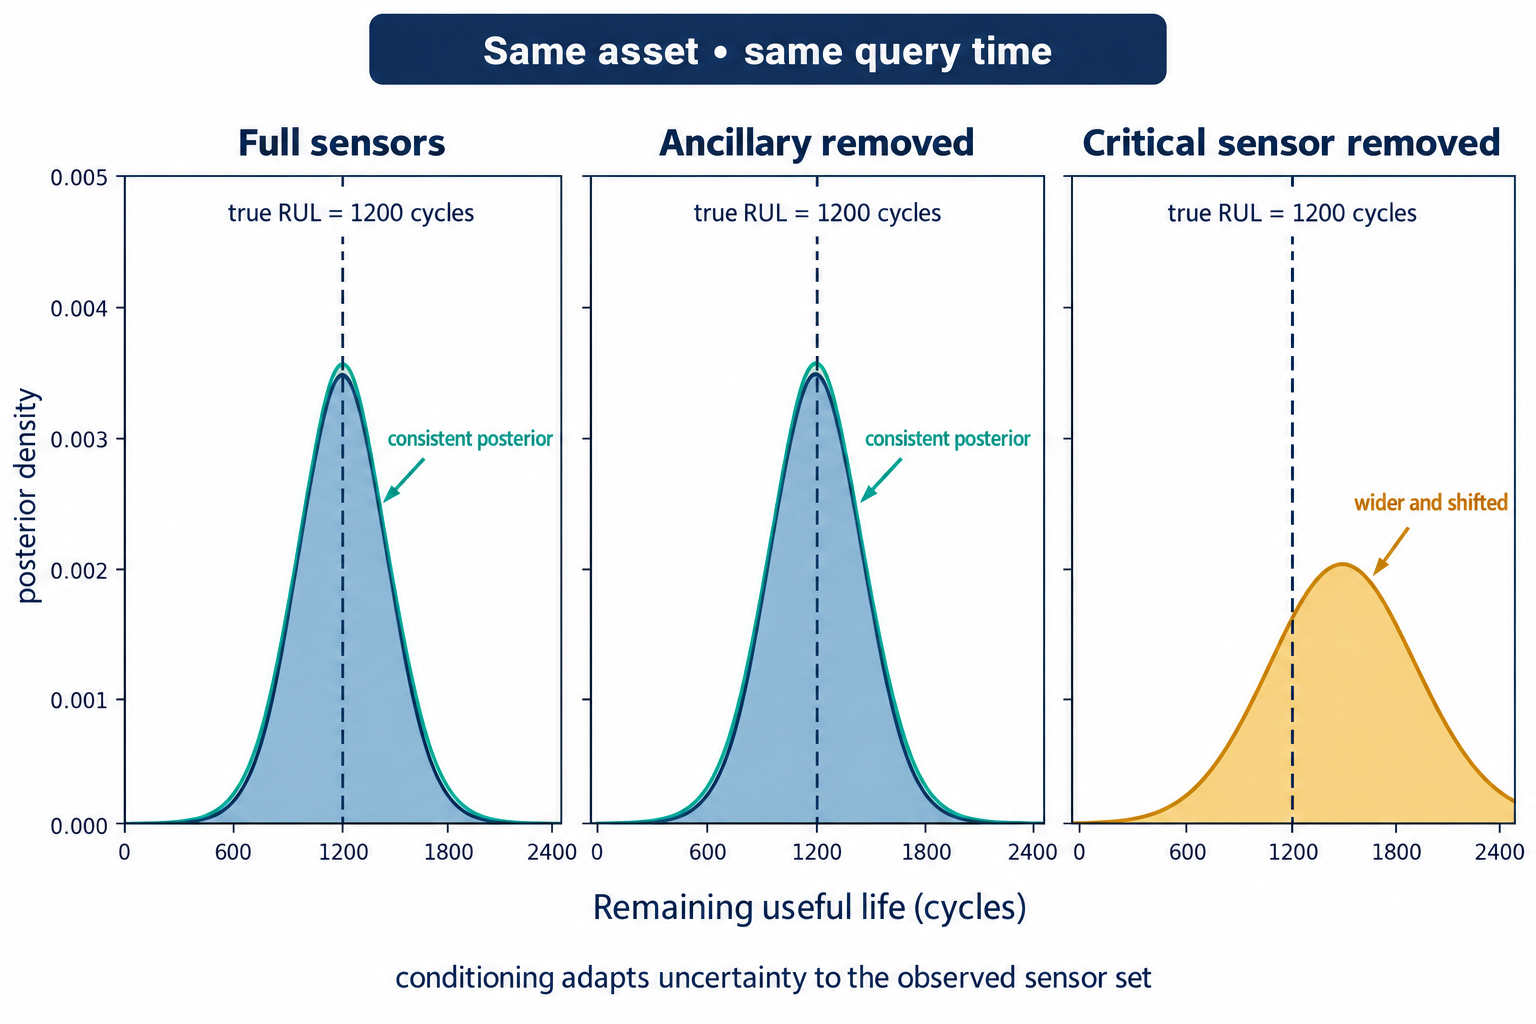
\includegraphics[width=0.86\linewidth]{fig6_prediction_example.png}
  \caption{\textbf{Illustrative prediction under changing sensor sets.} For the
  same asset and query time, full sensors and ancillary-sensor removal produce
  closely overlapping posteriors, while critical-sensor removal yields a wider
  and shifted distribution. The example gives an operational interpretation of
  cross-view consistency and its importance-dependent boundary.}
  \label{fig:prediction-example}
\end{figure}

\FloatBarrier

\subsection{Exploratory Mechanistic Analysis}
\label{sec:results:mechanism}

\subsubsection{Motivation and Scope}

The boundary-regime results suggest PROP-DIRECT can detect that information has changed (near-parity vs. full sensor complement) but struggles when functional importance matters (poor performance vs. matched random deletion). To investigate this mechanism, we conducted a post-hoc exploratory analysis examining how model predictions track oracle-defined task difficulty. This analysis was \emph{not} part of the pre-registered decision criteria and should be interpreted as hypothesis-generating rather than confirmatory.

\subsubsection{Oracle-relative geometry}

A low cross-view distance alone would also be achieved by a model that ignores
the sensor set and emits the same posterior for every view. We therefore use
the frozen oracle outputs to compute the secondary quantity
$E_{\mathrm{geometry}}=|d_{\mathrm{model}}-d_{\mathrm{oracle}}|$ for every paired
case. Table~\ref{tab:oracle_alignment} reports the asset-level summary for the
three deletion pair classes.

\begin{table}[tb]
  \centering
  \caption{\textbf{Exploratory oracle-relative geometry error on the C2 evaluation.}
  Values are asset-level means of $E_{\mathrm{geometry}}=|d_{\mathrm{model}}-d_{\mathrm{oracle}}|$;
  lower values indicate closer agreement with the oracle geometry. The final column
  reports the paired PROP-DIRECT minus B-STDPROB difference with a 90\% asset-bootstrap
  interval (2,000 replicates). This analysis is secondary and was not used in any
  preregistered decision rule.}
  \label{tab:oracle_alignment}
  \resizebox{\linewidth}{!}{%
  \begin{tabular}{lccc}
    \toprule
    Pair class & PROP-DIRECT & B-STDPROB & Difference [90\% CI] \\
    \midrule
    Critical vs. full & 0.0129 & 0.0129 & $+2.8\times10^{-5}$ $[-4.3\times10^{-4}, +4.9\times10^{-4}]$ \\
    Critical vs. matched random & 0.0134 & 0.0131 & $+3.7\times10^{-4}$ $[-4.3\times10^{-4}, +1.1\times10^{-3}]$ \\
    Critical vs. redundant & 0.0129 & 0.0127 & $+1.6\times10^{-4}$ $[-3.2\times10^{-4}, +6.2\times10^{-4}]$ \\
    \bottomrule
  \end{tabular}%
  }
\end{table}


The PROP-DIRECT and B-STDPROB errors are nearly indistinguishable for the
critical-versus-full comparison. PROP-DIRECT has a numerically larger residual
for the matched-random and redundant comparisons, but all paired 90\% intervals
include zero. This secondary analysis therefore makes the correctness question
explicit without turning it into a new superiority claim: the primary distance
result describes consistency, while $E_{\mathrm{geometry}}$ describes agreement
with the oracle-defined geometry.

\subsubsection{Oracle-Model Error Association}

For each prediction, we retained the oracle distance and the corresponding
oracle-relative geometry error. Figure~\ref{fig:b1-correlation} displays their
association for PROP-DIRECT across the three comparison types. Pearson
correlations are:

\begin{itemize}
    \item \textbf{Critical vs. Full:} $r = 0.5933$ ($n=119{,}232$)
    \item \textbf{Critical vs. Redundant:} $r = 0.5836$ ($n=119{,}232$)
    \item \textbf{Critical vs. Random:} $r = 0.5345$ ($n=19{,}872$)
\end{itemize}

\begin{figure}[!ht]
  \centering
  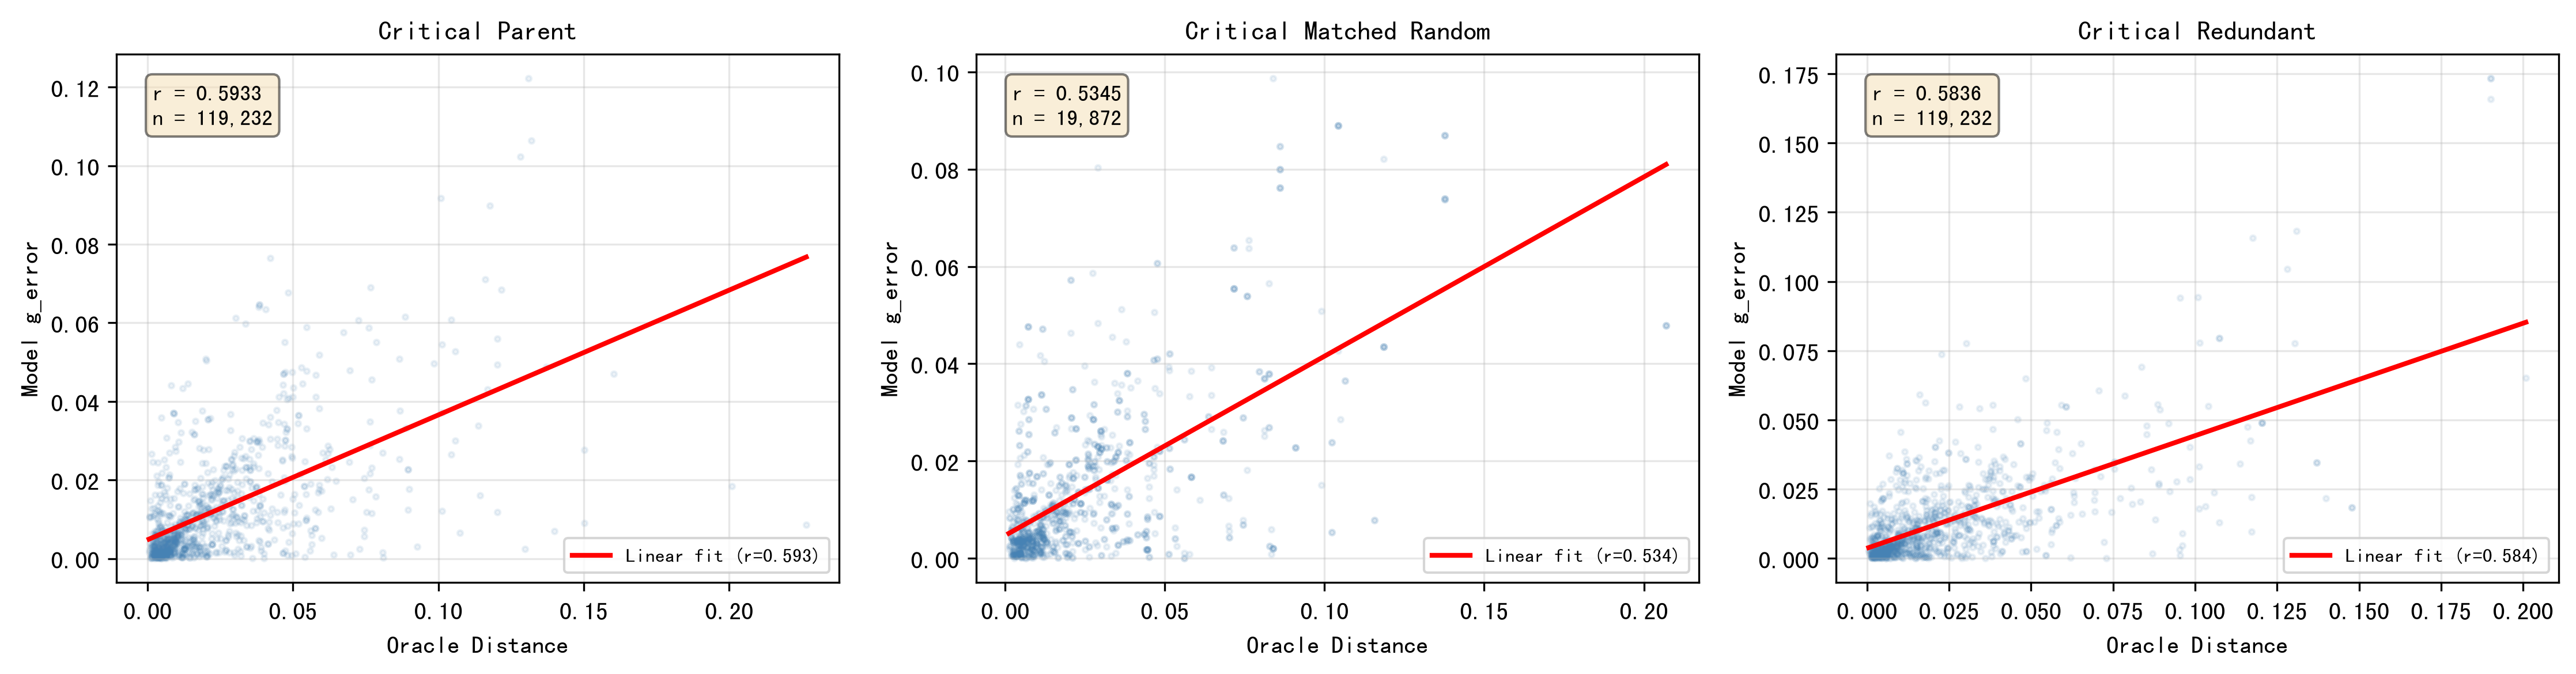
\includegraphics[width=\linewidth]{figures/b1_oracle_correlation_figure.png}
  \caption{\textbf{Oracle-relative geometry error across deletion pair classes.} Each panel shows the association between oracle distance and $E_{\mathrm{geometry}}=|d_{\mathrm{model}}-d_{\mathrm{oracle}}|$ for PROP-DIRECT across 1,000 randomly sampled test cases. Left: Critical vs. full sensor complement ($r=0.5933$). Center: Critical vs. matched random deletion ($r=0.5345$). Right: Critical vs. redundant deletion ($r=0.5836$). The correlations are descriptive because cases share assets and query structure; they do not establish a new confirmatory endpoint.}
  \label{fig:b1-correlation}
\end{figure}

The critical-vs-random association is 9.9\% weaker than the critical-vs-full association. We treat this contrast as an exploratory pattern in oracle-relative error; the paired cases share assets and query structure.

\subsubsection{Baseline Comparison: Architecture-Specific Limitation}

The standard baseline (B-STDPROB) exhibits the opposite pattern:
\begin{itemize}
    \item \textbf{Critical vs. Full:} $r = 0.6606$
    \item \textbf{Critical vs. Random:} $r = 0.6732$
\end{itemize}

For B-STDPROB, the matched-random correlation is stronger. The contrast associates the weaker-correlation pattern with PROP-DIRECT's sensor-set conditioning pathway rather than with prognostic models in general.

\subsubsection{Interpretation}

The residual analysis suggests that PROP-DIRECT approximates the oracle-defined geometry about as closely as the baseline in the critical-versus-full comparison, with a larger point estimate under matched-random deletion. Together with the pair-class ordering, this indicates that the availability signal is easier to represent than the functional distinctions among sensors. The evidence is diagnostic rather than a proof that either model has the correct posterior geometry in every case.

\subsection{Prediction Quality and Calibration}
\label{sec:results:quality}

\subsubsection{Predictive quality and posterior geometry}

We compared standard prognostic quality metrics across all seven model variants in the frozen model suite. Table~\ref{tab:c2_quality} reports asset-level macro-averages on the information-loss evaluation, which is scored under a separate frozen contract covering the full 96-asset population (Section~\ref{sec:methods:protocol}); it is distinct from the 10-asset test/lockbox partition used for the sufficient-observation claims.

\begin{table}[tb]
  \centering
  \caption{Descriptive predictive quality under information loss
  (covering the full 96-asset population; distinct from the 10-asset
  test/lockbox partition described in
  Section~\ref{sec:methods:protocol}). Values are means within asset followed
  by means over 96 assets; lower is better.}
  \label{tab:c2_quality}
  \resizebox{\linewidth}{!}{%
    \begin{tabular}{lrrrrrr}
      \toprule
      Model & State MAE & Failure MAE & CRPS & State rank & Failure rank & CRPS rank \\
      \midrule
      \propdirect{} & 0.014577 & 0.069585 & 0.048445 & 3 & 3 & 2 \\
      \bstdprob{}   & 0.014462 & 0.069195 & 0.048038 & 2 & 1 & 1 \\
      B-INDEP       & 0.014881 & 0.070197 & 0.049115 & 5 & 5 & 5 \\
      B-INVAR       & 0.014847 & 0.069970 & 0.048645 & 4 & 4 & 3 \\
      B-CDE         & 0.015563 & 0.070610 & 0.049103 & 6 & 6 & 4 \\
      B-SET         & 0.017344 & 0.071081 & 0.049566 & 7 & 7 & 7 \\
      B-WIDEN       & 0.014455 & 0.069255 & 0.049189 & 1 & 2 & 6 \\
      \bottomrule
    \end{tabular}%
  }
\end{table}


PROP-DIRECT ranks third for both state mean absolute error (MAE) and failure-time MAE, and second for CRPS among the seven models. Its CRPS difference from B-STDPROB is $+4.07 \times 10^{-4}$.

The quality table separates predictive accuracy from cross-view geometry: PROP-DIRECT remains competitive on single-view metrics even where its geometric advantage disappears. The C-MAPSS analysis next asks whether this distinction is visible on a public simulated benchmark.

\subsubsection{Posterior Calibration}
\label{sec:results:calibration}

We next use the frozen C1 posterior samples for a descriptive calibration check. The central intervals are close to their nominal levels on both held-out splits: the mean 90\% coverage across the three coordinates is 0.909 for PROP-DIRECT on test and 0.902 on lockbox, compared with 0.913 and 0.903 for B-STDPROB. The PIT histograms are likewise close to the uniform reference (Figure~\ref{fig:calibration}); the small differences do not support a claim that either method is uniformly better calibrated. This result separates the paper's primary geometric finding from posterior reliability: the conditioning mechanism improves cross-view geometry under sufficient observation while calibration remains broadly comparable to the baseline.

\begin{table}[tb]
\centering
\caption{\textbf{Posterior calibration diagnostics on the C1 evaluation splits.} Coverage entries are averaged over the three joint coordinates and include 90\% asset-bootstrap intervals. PIT histogram L1 is a descriptive distance from a uniform histogram; zero is ideal.}
\label{tab:calibration}
\begin{tabular}{llcc}
\toprule
Model & Split & 90\% coverage & PIT histogram L1 \\
\midrule
\propdirect{} & test & 0.909 [0.888, 0.928] & 0.082 \\
\propdirect{} & lockbox & 0.902 [0.877, 0.925] & 0.084 \\
\bstdprob{} & test & 0.913 [0.894, 0.931] & 0.084 \\
\bstdprob{} & lockbox & 0.903 [0.877, 0.927] & 0.085 \\
\bottomrule
\end{tabular}
\end{table}


\begin{figure}[!ht]
  \centering
  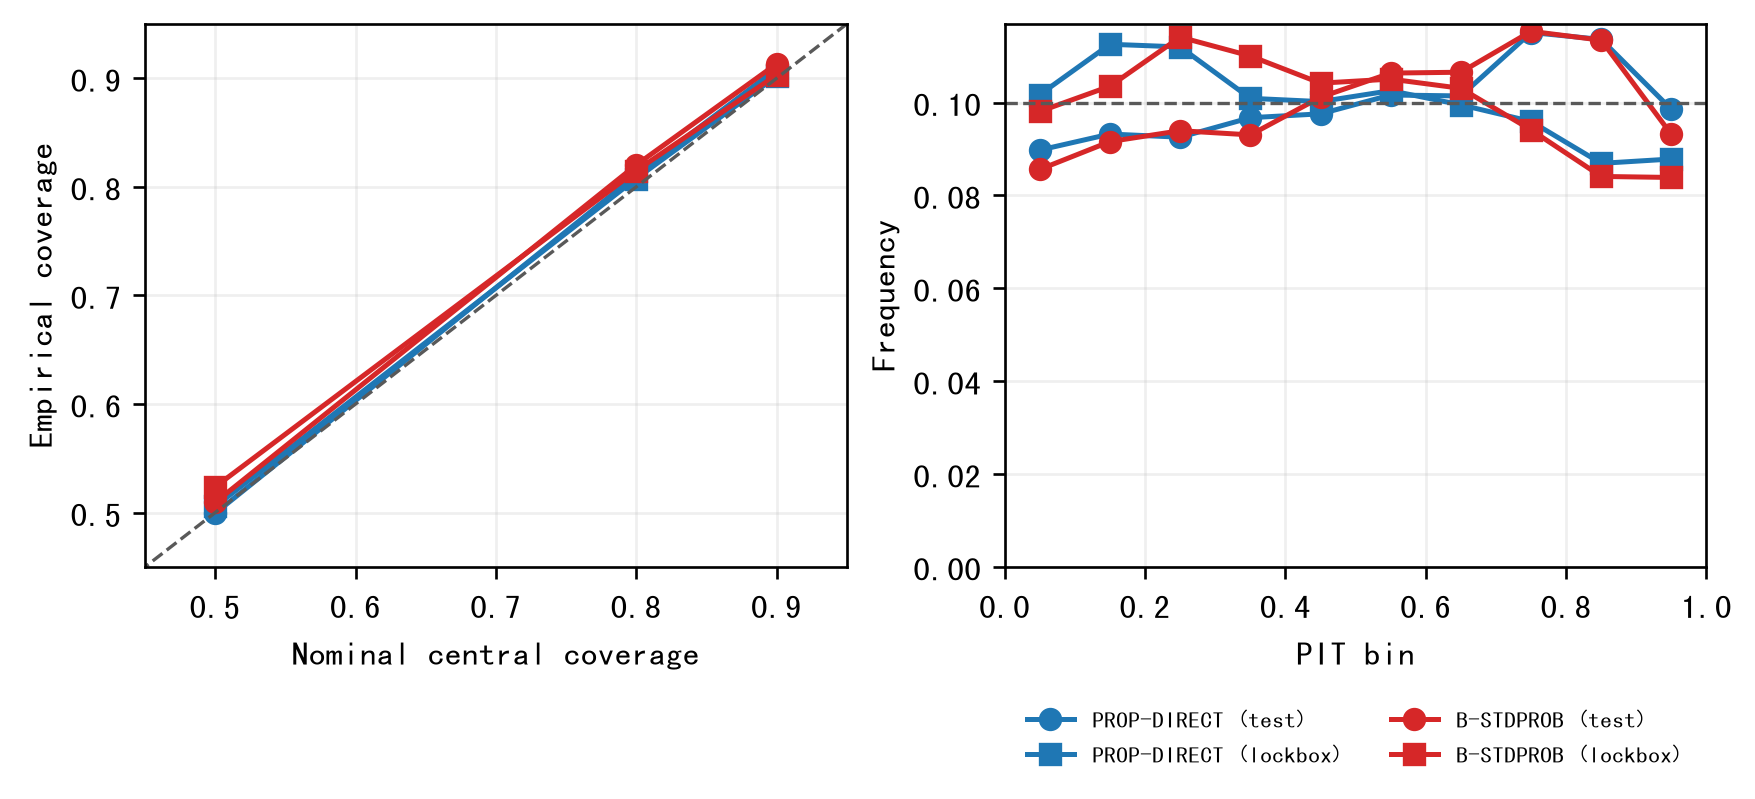
\includegraphics[width=0.94\linewidth]{fig7_calibration_reliability.png}
  \caption{\textbf{Posterior calibration diagnostics.} Left: empirical central coverage at nominal 50\%, 80\%, and 90\% levels, averaged over the three joint coordinates. Right: PIT histograms with the uniform reference shown by the dashed line. Circles and squares denote test and lockbox splits; the plots are descriptive checks rather than additional decision gates.}
  \label{fig:calibration}
\end{figure}

% Protocol-aligned benchmark evaluation. FD001 is simulated and uses artificial
% sensor deletion; it is reported as benchmark evidence rather than field validation.
\subsection{Conditional Cross-View Geometry on C-MAPSS}
\label{sec:results_cmapss}

To test the geometric hypothesis under the shared-model protocol, we evaluated PROP-DIRECT and B-STDPROB on C-MAPSS FD001~\citep{saxena2008cmapss}. FD001 contains 100 training and 100 test engine trajectories generated by NASA's Commercial Modular Aero-Propulsion System Simulation, with 14 non-constant sensor channels after preprocessing. It provides a public simulated reference for the analysis, while remaining distinct from field data.

\subsubsection{Shared-model protocol}

We retained the full 14-channel view and formed two reduced views by deleting three channels from each (11 channels per view; the two deletion sets differ by six channels). For each method, a single model was trained on the union of all three masked views. The 100 training engines were split by engine into 80 fitting and 20 validation engines, so views of the same engine remained in one split. The models use the MSE point-prediction head implemented for this benchmark; 128 dropout passes at test time provide predictive samples. We evaluate the final window of each of the 100 test engines and report energy distances on the raw RUL scale.

\subsubsection{Agreement depends on the view pair}

Table~\ref{tab:cmapss_validation} shows a conditional pattern. PROP-DIRECT reduces the distance to the full view by 18.5\% (90\% CI: 7.8--29.3\%) for View 1 and by 28.9\% (18.4--37.9\%) for View 2. For the two reduced views, however, the ordering reverses: PROP-DIRECT has a 36.6\% larger distance than B-STDPROB (90\% CI: $-62.9$ to $-13.1$\%). The shared model therefore aligns predictions when a reduced view is compared with the full sensor complement, but it does not maintain that alignment when two equally sized views differ in sensor identity.

% Table: C-MAPSS benchmark evaluation (shared-model regime, quality-controlled)
\begin{table}[t]
\centering
\begin{threeparttable}
\caption{\textbf{Cross-view energy distances on the C-MAPSS FD001 simulated
turbofan benchmark under the shared-model protocol.} A single model per
architecture is trained on data that mixes all three observation
configurations, mirroring the synthetic protocol. Lower energy distance
indicates closer agreement between dropout-sampled predictive distributions
for the same engine viewed under different sensor configurations; distances
are on the raw RUL scale (cycles). Bootstrap 90\% confidence intervals in
brackets (2,000 replicates, resampling engines). Negative relative reduction
indicates PROP-DIRECT is \emph{worse}.}
\label{tab:cmapss_validation}
\begin{tabular}{lccc}
\toprule
\textbf{View Pair} & \textbf{PROP-DIRECT} & \textbf{B-STDPROB} & \textbf{Relative Reduction} \\
\midrule
Full vs.\ View 1    & 1.85 [1.61, 2.11] & 2.27 [2.04, 2.51] & 18.5\% [7.8\%, 29.3\%] \\
Full vs.\ View 2    & 1.80 [1.56, 2.05] & 2.54 [2.29, 2.79] & 28.9\% [18.4\%, 37.9\%] \\
View 1 vs.\ View 2  & 1.85 [1.57, 2.17] & 1.36 [1.19, 1.52] & $-36.6$\% [$-62.9$\%, $-13.1$\%] \\
\bottomrule
\end{tabular}
\begin{tablenotes}
\footnotesize
\item Single-view test MAE (cycles), same runs: PROP-DIRECT 16.44 (full) /
15.95 (View 1) / 16.25 (View 2); B-STDPROB 16.27 (full) / 15.42 (View 1) /
15.73 (View 2). The near-identical point accuracy makes this geometry
comparison quality-controlled: differences in cross-view distance cannot be
attributed to differences in posterior informativeness.
\end{tablenotes}
\end{threeparttable}
\end{table}


The single-view MAEs are close across methods. PROP-DIRECT obtains 16.44, 15.95, and 16.25 cycles for the full, View 1, and View 2 conditions, compared with 16.27, 15.42, and 15.73 for B-STDPROB. The reversal in the reduced-view pair is consequently not explained by a large point-accuracy collapse. It is consistent with a more specific sensitivity to which sensors are present, although the benchmark has no oracle posterior with which to identify the mechanism.

This shared-model result is stronger evidence than the earlier specialist comparison because the conditioning pathway is trained across views, but it remains evidence from a simulated benchmark with artificial deletion. It supports a conditional extension of the synthetic finding and sharpens the importance-awareness boundary; it does not establish performance under naturally occurring sensor loss. The archived protocol and outputs make a future study with domain-informed critical channels and field data possible.


\section{Discussion}
\label{sec:discussion}

\subsection{What the Results Show}

The central result is a geometric one. When the available sensor views remain task-sufficient, explicitly conditioning the predictor on the observation process reduces disagreement between posterior predictions for the same asset. The 38.6\% reduction in cross-view energy distance is stable across the independent test and lockbox partitions and remains after a four-fold reduction in Monte Carlo samples. The effect therefore captures a property of the representation rather than a particular sampling budget.

The boundary experiment gives this result its meaning. Once functionally critical sensors are removed, PROP-DIRECT no longer preserves the same advantage. Its oracle-model correlation is 9.9\% weaker in the matched-random comparison, whereas B-STDPROB shows the opposite ordering. The cases are exploratory and share assets, so the correlation is best read as a mechanistic clue. The clue is nevertheless specific: the architecture responds to the amount of available information more readily than to the role played by an individual sensor. A model can therefore be geometrically stable across views while still being insufficiently sensitive to what has been lost.

This distinction separates two questions that are often combined in missing-sensor studies. The first asks whether predictions for one asset remain compatible as its observation set changes. The second asks whether the model recognizes that different missing sensors can have different consequences. The present architecture addresses the first question under task sufficiency and exposes the second as its current boundary.

\subsection{An Architectural Interpretation}

PROP-DIRECT supplies the model with a representation of the available sensor set alongside the observed sequence. This gives the predictor a direct route to adjust its posterior geometry when the observation process changes. It also creates a demand on that representation: the set description must preserve distinctions that matter for degradation. The matched-random result suggests that the current flat representation does not reliably preserve those distinctions when sensor importance is strongly heterogeneous.

The baseline provides a useful comparison because it has no explicit sensor-set input. Its stronger matched-random correlation is consistent with a more conservative response to missing observations: broad uncertainty may track the severity of a critical deletion better than a configuration-specific adjustment that lacks an importance signal. This explanation is plausible rather than identified by the present experiments. It motivates a design principle for the next model generation: condition on availability, but give the conditioning pathway a structured account of sensor function.

Hierarchical representations could separate subsystem status from individual sensor status; state-dependent attention could allow importance to change with degradation mode; and physics-informed priors could encode known functional roles. These are extensions of the same geometric objective, rather than replacements for it. They should be evaluated with both sufficient-view consistency tests and deletion tests that hold sensor count fixed while changing functional importance.

\subsection{Relation to Existing Prognostic Practice}

Imputation and missing-data methods~\citep{rubin1976inference,little2019statistical,che2018gru,cao2018brits,tashiro2021csdi} primarily reconstruct an unobserved measurement before making a prediction. Observation-process conditioning keeps the availability event explicit, allowing uncertainty about the observation process to remain visible in the posterior. The results here suggest that the two ideas are complementary: imputation may recover information from a critical channel, while conditioning can maintain a coherent geometry across the views that remain.

Set encoders and attention mechanisms~\citep{lee2019settransformer,vaswani2017attention,zaheer2017deep} provide natural alternatives for representing variable sensor collections. Their presence in a model does not by itself establish importance awareness. A meaningful comparison should therefore pair standard point and probabilistic accuracy with the cross-view and matched-random tests used here. Multi-task or meta-learning objectives~\citep{finn2017model} could further supply training signals for configurations that a single shared model must serve.

\subsection{The C-MAPSS Result in Context}
\label{sec:limitations}

The synthetic generator gives the primary experiment a property that field data cannot easily provide: an exact oracle posterior and direct control over which observation process is applied to the same latent asset. C-MAPSS FD001 offers a complementary public reference point, but it is also a simulated benchmark. In the shared-model evaluation, one predictor per method was trained on all three views, the predictors used an MSE point head with dropout sampling, and each reduced view was formed by artificial deletion of three of the 14 active channels.

The result is conditional. PROP-DIRECT reduces distance to the full view by 18.5--28.9\%, but is 36.6\% worse than B-STDPROB for the pair of equally sized reduced views. Single-view MAE is close across methods, so the reversal does not track a broad point-accuracy collapse. The pattern is consistent with sensitivity to sensor identity that remains incomplete under the current representation. It is protocol-aligned evidence from a simulated benchmark, not field validation; data with naturally occurring sensor loss would test whether the same boundary matters in operation.

\subsection{Scope and Future Tests}

Several aspects of the evidence define the next experiments rather than weaken the result already established. The synthetic study uses one generator family and focuses on RUL posterior geometry; the calibration diagnostic is broadly comparable between methods, but replication with independent generators, tail-risk metrics, and other prognostic tasks would test the breadth of the finding. The present model comparison also leaves attention-based, ensemble, and importance-aware architectures open. These comparisons are especially valuable because a model that is accurate in a single view can still be poorly aligned across views, while a model that is highly aligned can achieve that agreement by becoming insufficiently informative.

For practical evaluation, the most informative sequence is therefore straightforward: first train a shared model across observation configurations on the public benchmark, then repeat the deletion study with domain-informed critical channels, and finally examine longitudinal assets with naturally occurring outages. If these tests preserve the geometry gain while improving the importance boundary, observation-process conditioning would offer a useful component for uncertainty-aware maintenance decisions. If they do not, the present study still identifies the relevant failure mode and the metric pair needed to detect it.

\section{Conclusion}
\label{sec:conclusion}

Reliable prognostics must remain coherent when the sensors available to an asset change. In a controlled synthetic evaluation with exact oracle posteriors, explicitly conditioning the predictor on the observed sensor set reduced cross-view posterior inconsistency by 38.6\% (90\% CI: 34.8--42.4\%) when the alternative views remained task-sufficient. The effect persisted after a four-fold reduction in Monte Carlo sampling, suggesting that the gain is tied to the representation of the observation process rather than to a large sampling budget.

The same study identifies the boundary of that gain. Under permanent removal of functionally critical sensors, PROP-DIRECT did not retain its advantage, while exploratory oracle-model correlations showed a weaker distinction between critical and random deletions than the standard baseline. These comparisons are descriptive because the cases share assets and query structure, but they point to a concrete architectural issue: recording which sensors are present is easier than representing what those sensors mean for the degradation process. The result is a useful design constraint for future importance-aware conditioning, rather than a reason to discard observation-process conditioning altogether.

On C-MAPSS FD001, the shared-model evaluation reduces distance to the full view by 18.5--28.9\%, but increases the distance between the two equally sized reduced views by 36.6\%. Point MAE remains close to the baseline. This conditional pattern extends the geometric result to a public simulated benchmark while sharpening the importance-awareness boundary; evaluation with naturally occurring sensor loss remains the next test.

Taken together, the findings support a simple principle for probabilistic prognostics: observation-process conditioning is valuable when available views preserve the information needed by the task, and it needs an explicit account of functional importance when they do not. Hierarchical sensor representations, state-dependent importance weights, and physics-informed priors offer natural ways to pursue that account while retaining the geometric objective introduced here.


\section*{Data Availability Statement}

The synthetic generator used in this study is based on controlled degradation models that enable exact oracle posterior computation. Complete generator specifications, evaluation scripts, protocol documents, and compact result artifacts are available in the public repository. Due to the pre-registration protocol, all evaluation code was frozen prior to accessing lockbox validation data. The repository includes:

\begin{itemize}
    \item Synthetic data generator with seed specifications for replication
    \item Shared-model C-MAPSS training and evaluation scripts with configurations and results
    \item Calibration analysis code, coverage/PIT summaries, and the reliability figure
    \item Compact scoring outputs and decision documentation; large prediction stores and checkpoints can be regenerated from the recorded protocols
    \item Pre-registration documents including frozen thresholds and decision rules
\end{itemize}

The public code and manuscript repository is available at
\url{https://github.com/xyforge/sensor-set-conditioning-rul}. It contains the
manuscript source, evaluation scripts, frozen protocol documents, compact
result summaries, and the shared-model C-MAPSS report. Raw C-MAPSS data and
large prediction stores are excluded and must be obtained or regenerated under
their respective data-access conditions. A persistent DOI can be added when a
versioned release is deposited in a research repository.

\section*{Acknowledgements}

This research was conducted under a preregistered protocol with independent test and lockbox evaluation splits. We thank the reviewers for their constructive feedback. C-MAPSS turbofan data were provided by NASA Ames Prognostics Center of Excellence. Computational resources were provided by institutional high-performance computing facilities. All experimental decisions were made prior to accessing validation outcomes to ensure statistical integrity.

\section*{Conflict of Interest Statement}

The authors declare no competing financial interests or personal relationships that could influence the work reported in this paper.

\bibliographystyle{elsarticle-num}
% Only cited entries appear in the bibliography. Uncited .bib entries are
% excluded until integrated into the text (reviewer issue P2: bibliography
% previously padded via \nocite{*} but not cited in body).
\bibliography{references}

\end{document}
